% \documentclass[sigconf, anonymous]{acmart}
\documentclass[sigconf]{acmart}

\usepackage{booktabs} % For formal tables
\usepackage{graphicx}
% Note: do not use url & hyperref packages.
% They do not pass the IEEE pdfxpress checks
% \usepackage{url}
% \usepackage{hyperref}
% \usepackage{subfigure}
\usepackage{balance}
\usepackage{amssymb,amsmath}
% \usepackage[usenames,dvipsnames,svgnames,table]{xcolor}
\usepackage{algpseudocode}
\usepackage{todonotes} % get rid of this later
\usepackage{subfig}

\newcommand{\compactimg}{\vspace{-10pt}}
\newcommand{\tableref}[1]{Table~\ref{tab:#1}}
\newcommand{\figref}[1]{Figure~\ref{fig:#1}}
\newcommand{\secref}[1]{Section~\ref{sec:#1}}
\newcommand{\algoref}[1]{Algorithm~\ref{algo:#1}}

\newcommand{\bob}[1]{\textcolor{red}{{\bf from Bob: #1}}}


\newenvironment{tightitem}{\begin{itemize}\setlength{\itemsep}{1pt}\setlength{\parskip}{0pt}\setlength{\parsep}{0pt}}{\end{itemize}}

% Copyright
%\setcopyright{none}
%\setcopyright{acmcopyright}
%\setcopyright{acmlicensed}
\setcopyright{rightsretained}
%\setcopyright{usgov}
%\setcopyright{usgovmixed}
%\setcopyright{cagov}
%\setcopyright{cagovmixed}


% DOI
\acmDOI{None}

% ISBN
\acmISBN{}

%Conference
\acmConference[SenSys'17]{ACM Conference on Embedded Networked Sensor Systems}{2017}{Delft} 
\acmYear{2017}
\copyrightyear{2017}

\acmPrice{xx.00}

\title{Location-Aware Network Management for LoRa \\ Low-Power Wide Area Networks}


%\titlenote{Produces the permission block, and
%  copyright information}
% \subtitle{Extended Abstract}
% \subtitlenote{The full version of the author's guide is available as
%   \texttt{acmart.pdf} document}

% No clue why  this doesn't work or where the current Author is coming from.  Also seems to be a maketitle warning
\author{Paper Number 202}
%\author{\vspace{1cm}Paper Number 202}
%\affiliation{%
%  \institution{Anonymous Institution}
%  \streetaddress{P.O. Box 1234}
%  \city{City} 
%  \state{State} 
%  \postcode{12345}
%}
%\email{anon@anon.com}

% The default list of authors is too long for headers}
%\renewcommand{\shortauthors}{Anonymous et al.}

\begin{document}

\begin{abstract}
Low-Power Wide Area Networks (LP-WANs) are an emerging wireless platform designed to enable long-range communication at low data rates to tens of thousands of battery-operated sensing devices. Unlike in cellular networks where towers are strategically placed, the uncoordinated nature of LP-WANs compounded with their long transmission range can yield poor overall network capacity. In this paper, we explore the management of multiple LP-WAN base stations using LoRa radios that operate in unlicensed sub-GHz spectrum. Due to FCC regulations, these devices are required to hop across several frequencies. We exploit this frequency hopping requirement along with the massive scale in terms of number of clients to provide both device localization and spectrum sensing that can be combined to improve overall network capacity.

LP-WAN devices are designed to be low-power and therefore operate over limited bandwidths (a few hundred kHz), which limits localization accuracy to hundreds of meters. We introduce a technique that stitches together multiple channels as the device hops across frequencies to emulate a wider bandwidth radio with positioning errors on the order of few meters. At scale, this improved localization along with the required channel hopping allows us to create a live heat-map of signal quality across the environment. We show that this comprehensive spectrum sensing can then be used to optimize a team of coordinating base stations and clients to both improve its own performance while also coexisting with networks outside of its control.  We also show the potential increase in capacity, when clients near gateways are scheduled on whitespace frequencies that are accessible by LoRa hardware. Through a mixture of experimentation and simulation, we demonstrate how our system maps client devices to appropriate frequencies, transmits power levels and base station information in a manner that improves load balancing, reduces interference, and increases throughput.
\end{abstract}

%
% The code below should be generated by the tool at
% http://dl.acm.org/ccs.cfm
% Please copy and paste the code instead of the example below. 
%
%\begin{CCSXML}
%<ccs2012>
%  <concept>
%   <concept_id>10010520.10010553.10010562</concept_id>
%   <concept_desc>Computer systems organization~Embedded systems</concept_desc>
%   <concept_significance>500</concept_significance>
%  </concept>
%  <concept>
%   <concept_id>10010520.10010575.10010755</concept_id>
%   <concept_desc>Computer systems organization~Redundancy</concept_desc>
%   <concept_significance>300</concept_significance>
%  </concept>
%  <concept>
%   <concept_id>10010520.10010553.10010554</concept_id>
%   <concept_desc>Computer systems organization~Robotics</concept_desc>
%   <concept_significance>100</concept_significance>
%  </concept>
 
% <concept>
%  <concept_id>10003033.10003083.10003095</concept_id>
%  <concept_desc>Networks~Network reliability</concept_desc>
%  <concept_significance>100</concept_significance>
% </concept>
%</ccs2012>  
%\end{CCSXML}

%\ccsdesc[500]{Computer systems organization~Embedded systems}
%\ccsdesc[300]{Computer systems organization~Redundancy}
%\ccsdesc{Computer systems organization~Robotics}

%agr removed \ccsdesc[100]{Networks~Network services}

% We no longer use \terms command
%\terms{Theory}

%\keywords{low-power wide area networking, systems, localization, wireless, network management, LoRaWAN}


\maketitle


\section{Introduction}
\label{sec:intro}

Low Power Wide Area Networks (LPWANs) are increasingly seen as an attractive
communication platform for city-scale Internet-of-Things (IoT) deployments.
They offer the ability to wirelessly connect energy-constrained devices to
gateways over distances of many kilometers. LPWANs also have power and cost
advantages over alternatives like cellular networks, particularly in
deploy-once, low maintenance and low throughput sensing applications.

While LPWANs are far from pervasive, the capabilities of networks like
LoRaWAN~\cite{Sornin2015, LoRaWanAlliance2015}, SigFox~\cite{centenaro2016}
and Ingenu's RPMA~\cite{Ingenu2015} have attracted investment and have spawned
early deployments. These technologies operate on the unlicensed ISM spectrum,
allowing businesses and consumers alike to deploy their own devices and
gateways. With Comcast recently announcing integration of LPWAN radios into
future set-top boxes in the U.S.~\cite{comcast2}, LPWANs are likely
to grow rapidly. Given that each LPWAN gateway promises a range of up to ten
kilometers~\cite{LoRaWanAlliance2015}, major cities are likely to see a
fast-paced expansion in LPWAN coverage.

Despite the expected rise in density of LPWAN gateways, not all devices will
experience the promised 10 year battery life. Devices located in urban spaces
deep inside buildings or in remote neighborhoods will experience severe drain
in battery as their signals are highly attenuated even at the closest base
station. Some of these devices, such as those in basements or tunnels, may not
be in communication range of any gateway at all. Unlike cellular networks,
LPWANs are largely user-deployed and unplanned, meaning that these devices may
remain battery deprived or simply out of network reach in perpetuity, even as
thousands of gateways proliferate city-wide.

\begin{figure}[tb]
    \centering
    % \vspace{-10pt}
    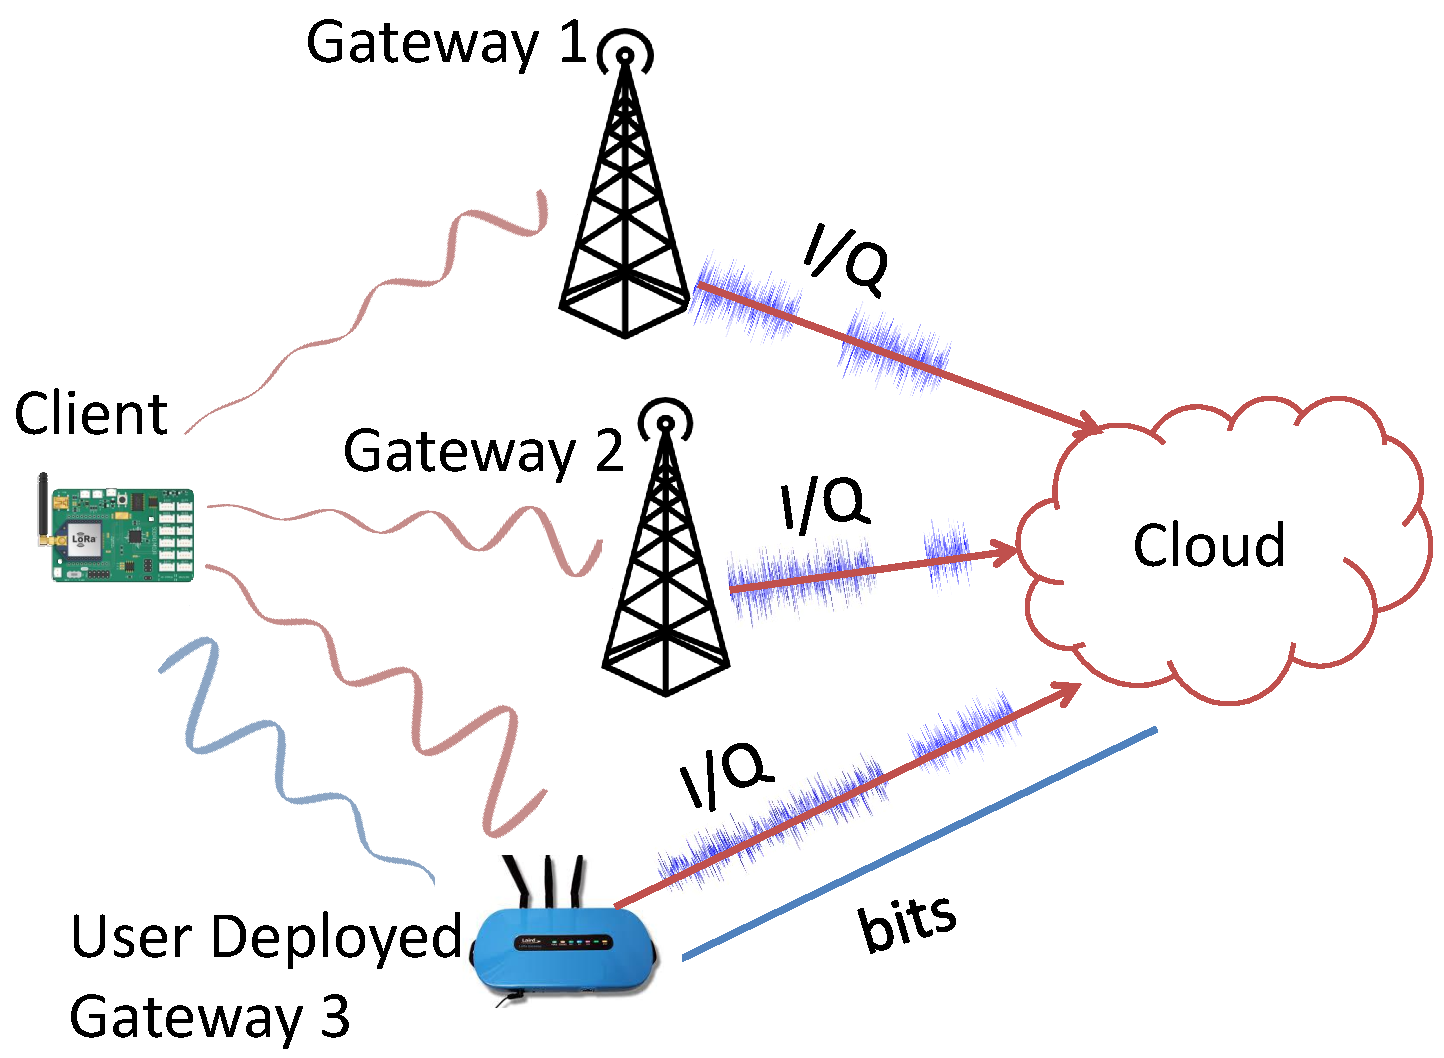
\includegraphics[width=0.60\columnwidth]{figures/LoRaRAN_cropped}
    \vspace*{-10 pt}
    \caption{Charm: LPWAN joint decoding in the cloud}
    \compactimg
    \label{fig:my_label}
\end{figure}

This paper presents Charm, a system that enhances the coverage of LPWANs and
the battery life of client devices in large urban deployments. Charm exploits
the observation that while signals from certain clients may attenuate
significantly, they are still likely to be received by multiple gateways in a
dense network. Charm introduces a hardware and software design at the gateways
that identifies and transports weak received signals to the cloud. We then
develop a joint decoding system at the cloud that coherently combines weak
signals received across multiple city gateways to decode the underlying data.
As a result, Charm both expands the decoding range of the LPWAN network and
improves battery-life for nodes already in range -- allowing client devices to
spend less energy per transmitted bit. Charm is built on the LoRaWAN
platform~\cite{LoRaWanAlliance2015}, a popular and widely available LPWAN
technology. Charm is implemented in a first-of-its-kind pilot deployment for
coherent diversity combining and demonstrates increased network coverage and
improved data rates across client devices.

While coherent diversity combining and PHY-layer processing in the cloud has
received much attention in the Wi-Fi~\cite{tan2009sam, xie2014scalable} and
cellular~\cite{checko2015cloud, wubben2014benefits} context, designing such a
system for low-power WANs offers radically new challenges. At the gateways, we
would have to decode very weak signals, weaker than 30 dB below the noise
floor. Simply uploading all received data to the cloud would overwhelm
the backend link, which is often  a simple home LAN. Both the LPWAN gateways
and clients are designed to be economical and deployed at scale, and without
the time synchronization required for coherent combining. At the cloud,
collating receptions from a large number of gateways at city-scale to identify
which of them contain packets from the same client is a challenge. We provide
an overview of our approach to address each of these challenges.

\noindent \textbf{Noise-Resilience at the Gateway:} The key challenge at the
gateway is identifying packets that are significantly below the noise floor
and, therefore, virtually undetectable. A straw-man approach to this problem
would be to correlate the received signal with a known preamble in any valid
packet. For instance, LoRaWAN uses a sequence of identical chirps -- signals
whose frequency increases linearly in time -- as a signature that is prefixed
in every packet. In principle, sending an extremely long preamble could
provide high resilience to noise. In practice, doing so goes against the
spirit of LPWANs where energy for transmission is a valuable resource for the
client.

Charm's approach to resolving this challenge is a hardware and software gateway
design that leverages the structure of the LoRaWAN LPWAN protocol.
Specifically, we develop a transform that converts the data symbols containing
\textit{a priori} unknown bits into a repeated and known sequence of signals,
much like the preamble. Charm can therefore now use both the preamble and the
modified data sequence to detect any packet.

To understand our approach at a high-level, we present an illustrative example
that dives into the details of the LoRaWAN PHY-layer. LoRaWAN transmits data
symbols as chirps whose initial frequency is a function of the data. For
instance over a bandwidth of 100 Hz, LoRa could represent the bit "0" as a
chirp starting at 2 Hz and bit "1" as a chirp starting at 52 Hz. Charm's
filter aliases the received LoRa signal so that frequencies modulo 50 Hz fold
into each other. This means that both bit "0" and bit "1" now map to an
identical chirp starting at 2 Hz. We apply this filter through the received
packet to obtain a repeated sequence of chirps as long as the entire packet
itself. This technique allows us to detect the packet with a much higher
resilience to noise compared to using the preamble alone, without incurring
additional overhead.

We develop a custom gateway hardware platform integrating a Semtech LoRaWAN
radio frontend, a low-power FPGA and Raspberry PI that can filter and detect
weak signals by processing received raw I/Q samples in real-time. Our hardware
platform, a hybrid between a full SDR and a dedicated high-performance radio,
is designed to be open and highly programmable -- a novel tool to experiment
with alternative LPWAN PHY-layer designs in the 900 MHz ISM band, without
compromising on signal quality or real-time performance.

\noindent \textbf{Scalability at the Cloud:} At the cloud, Charm must deal
with a large number of receptions from various gateways in a city, pruning for
weak signals and identifying common signals between gateways. Charm proposes
multiple optimizations to run its algorithms seamlessly at city-scale. For
instance, it is often the case that gateways transmit weak signals to the
cloud for packets that have already been decoded perfectly at other gateways.
However, realizing that the weak signal has already been decoded elsewhere is
impossible without decoding it in the cloud in the first place. Charm resolves
this chicken-or-egg dilemma by exploiting the timing and geographical location
of the received signal. Prior to sending any signal data to the cloud, a Charm
gateway sends the location, frequency, accurate timing and signal-to-noise
ratio (SNR) of the received weak packet. The cloud collates such information
across multiple gateways and requests for signals only from the gateways that
receive these signals the best. In doing so, Charm saves valuable uplink
bandwidth at the gateways and compution at the cloud. We describe how Charm
mitigates range of other important challenges at the cloud such as imperfect
timing, frequency offsets and overlapping transmissions.

We evaluate Charm in both indoor and outdoor environments using two testbeds
on the Carnegie Mellon University campus and around the city of Pittsburgh.
Eight user-deployed gateways built using our custom hardware platform support
a testbed covering a 0.6 sq.km. area around campus, which is used to study
Charm's performance with regard to local packet detection, range and
data-rates. Four rooftop gateways support the OpenChirp LPWAN network which
services a large 10 sq.km. area that we use to acquire traces for large-scale
simulations. Our results reveal the following:

\begin{itemize}
    \item {\bf Battery-Life: } By coherently combining across 8 base stations,
        Charm improves the SNR of a typical LoRaWAN transmission by 3.16 dB,
        extending battery life by up to 4$\times$.
    \item {\bf Range: } We improve the maximum communication range of 8 indoor
        user-deployed gateways in urban settings from 60m in LoRaWAN to 200
        meters using Charm, an overall increase in coverage area by
        10$\times$.
    \item {\bf Coverage: } Our trace-driven simulation, based on city-wide
        drive tests, estimates an overall increase in coverage area by up to 2x due
        to Charm over LoRaWAN.
\end{itemize}

\noindent \textbf{Contributions:} We make the following novel contributions:
\begin{itemize}
    \item A technique that leverages the geographical diversity of unplanned,
        user-deployed gateways to enable joint decoding of weak transmissions.
        This improves battery-life for users in the network and increases the
        coverage area.
    \item A hardware platform and the underlying algorithms for detecting weak
        LoRaWAN transmissions locally at the gateway.
    \item A software architecture that builds atop of LoRaWAN to enable
        joint-decoding of signals in a scalable manner.
\end{itemize}
\section{Related Work}
\label{sec:related-work}

% {\color{blue}
% [ANYTHONY, SWARUN, BOB, ARTUR, ADWAIT, DIANA, MAX]

% Particular topics to consider
% \begin{itemize}
% \item PerCom workshop paper
% \item Localization (Reverse GPS)
% \item WiFi and Cellular existing work
% \end{itemize}
% }

\noindent \textbf{Low-Power Wide-Area Networks: } Recent years have seen much
interest in Low-Power wide area networks (LP-WANs), including the development
of new hardware and standards. Private enterprises such as
Semtech~\cite{LoRaWanAlliance2015} and
SigFox~\cite{sanchez2016state} have developed LP-WAN chipsets that use extremely
narrow bands of unlicensed spectrum. In contrast, cellular standardization
bodies have developed two standards for LP-WAN communication for cellular base
stations to communicate with low-power IoT devices over licensed spectrum:
LTE-M~\cite{GSMAssociation2016} 
and NB-IOT~\cite{ratasuk2016nb}. 
Unlike LoRa and
SigFox, these technologies require devices to periodically wake up to
synchronize with the network -- a burden on battery life.

Several recent measurement studies have been conducted to evaluate the
performance and range of LP-WAN networks~\cite{petric2016measurements, toldov2016performance} and perform theoretical capacity
analysis~\cite{mikhaylov2016analysis}. Early pilot deployment efforts are also
underway with SigFox deploying their hardware to connect security alarms to
the cloud in Spain~\cite{sanchez2016state}, smart blood refrigerators in the
Democratic Republic of the Congo~\cite{ramachandranmupnp} and smart city
applications \cite{centenaro2015long}. These efforts motivate the challenge of
limited range, performance and battery-drain of LP-WAN clients. A recent system, Choir~\cite{eletreby2017empowering} has demonstrated improving range and scalability of LP-WANs through collaborations of weak client radios. In contrast, this paper seeks to use collaboration between gateways without any modifications to client behavior whatsoever to improve the battery life of even a single client. \\\vspace*{-0.1in}

\noindent \textbf{Distributed MIMO and Coherent Combining: } A large body of work has proposed the use of multiple-antennas (MIMO) to improve SNR and reduce interference~\cite{xie2014scalable, lin2011random, kumar2013bringing}. In the Wi-Fi context, past systems have used multi-user MIMO to improve performance on the uplink~\cite{shen2014rate, tan2009sam, xie2014scalable}. In the cellular context, massive MIMO proposals have demonstrated scaling gains of towers with a large number of antennas~\cite{shepard2012argos, larsson2014massive}. There has been much theoretical work on distributed MIMO overall in both the sensor networking context~\cite{del2007cooperative} and wireless LANs~\cite{dohler2004resource} and cellular networks~\cite{sawahashi2010coordinated}.  More recently, practical distributed MIMO systems, primarily in the LAN-context have demonstrated both multiplexing and diversity gains~\cite{hamed2016real, yenamandra2014vidyut, rahul2012jmb}. Instead, our approach brings the diversity gains of distributed MIMO on the uplink to low-power wide-area networks. In doing so, we overcome multiple challenges owing to the fact that signals at any individual tower are well below the noise floor. \\\vspace*{-0.1in}


\noindent \textbf{Cloud Radio Access Networks (Cloud-RAN): } Multiple research efforts from the industry and academia have advocated the use of PHY layer processing at the cloud as opposed to the base stations~\cite{sabella2013ran, hadzialic2013cloud}. In the cellular context, CloudRAN aims to perform baseband processing at the cloud, allowing base stations to be simple and easy to deploy~\cite{checko2015cloud, wubben2014benefits}. The key challenge however is the need for a reliable fiber optic backhaul to the cloud to collate data streams in a low latency manner, motivating the need for cost-effective high-performance backhauls~\cite{liu2013case, chih2014recent}.  Our approach aims to bring PHY processing in the cloud to low-power wide-area networks that operate at significantly lower bandwidth, with loose latency bounds and can therefore afford Ethernet backhauls. We perform a wide variety of optimizations to minimize the use of uplink bandwidth, even if the gateways are user-deployed with residential internet backbones. 



%{\color{blue} Discuss how we overcome some of cloud-RAN challenges due to short and infrequent messages}
\section{Motivation}
\label{sec:net-scale}

{\color{blue} A quick introduction to LoRa.... Check if we need more details about a particular aspect.}

LoRa offers a unique collection of features for dynamic data-rate selection and concurrent reception of packets on the gateway. In the U.S., LoRaWAN standardized 64 channels of downlink (125$khz$) and 8 channels of uplink (500$Khz$) per base station. Current gateways use the Semtech SX1301 base band processor which can listen on up to 8 channels at the same time. Most gateway hardware pairs the SX1301 with two radio frontends that each have four programmable reception channels. Each radio front-end listens across 800$kHz$ of bandwidth which supports up to four independent 125$kHz$ channels or a single 500$kHz$ channel (usually used for uplink).  The two radios can be configured independently such that one operates on the 433$MHz$ band while the other at 900$MHz$ which allows for both a large bandwidth span as well as whitespace coverage.  LoRaWAN specifies 7 spreading factors per channel (SX1301 supports 6) that in a similar spirit to CDMA, allows for multiple packets at different rates to be received simultaneously on the same channel.  Each increase in spreading factor leads to a doubling of transmission time but a 3.5$dB$ increase in link budget (i.e. range).  FCC regulations allow LoRa radios to operate in {\em hybrid-mode} where they can hop across a reduced subset of the total LoRaWAN channel set (8 sequential channels instead of 64). We refer the reader to \cite{sx1301} for a more detailed description of LoRa radio hardware capabilities.

{\color{blue} Some whitespace discussion would follow...}

% These parameters, along with FCC regulations for LoRa provide several degrees of freedom that can be used to optimize network performance in four main ways.  First, Adaptive Data Rate (ADR) algorithms can be used to improve network capacity by configuring power levels and selecting spreading factors.  Second, most standard base stations operating in hybrid-mode which can be coordinated across a network to avoid interference and collisions.  Third, clients can coordinate with the infrastructure to more intelligently select a base station to associate with, based on estimated load and spreading factors. In cases of high client density, we see that reducing data rate by shifting clients to slower spreading factors can lead to improved overall capacity. Finally, powered clients can help localize uncoordinated base stations or noise sources that the network can avoid.

Since LoRa radios can span a wide frequency range, we can also access available whitespace depending on the region and usage schedules.  Whitespace access requires location information for registering with spectrum databases and requires an out-of-band mechanism (like LoRa) as part of the join processes.  This makes it an ideal mechanism for offloading traffic in support of scale.

% In the rest of this section, we evaluate the potential to exploit the above techniques to improve overall network capacity. We first experimentally profile the LoRa channel in terms of interference between channels and spreading factors.  Next, we look at how base stations can be more efficiently managed and how clients can more efficiently be allocated to them.  We then show an initial mechanism that leverages our localization approach to perform impact assessment for noise sources.

% [ANTHONY, ADWAIT, MAX, ARTUR]

% \subsection{An Additive Interference Model}
% \label{sec:AIM}

% {\color{red} These effects don't seem to matter much once we consider probabilities.}

% A fundamental property of wireless communication is the use of a shared medium, in which the reception of a signal can be affected by the transmission of other unrelated signals. A wireless receiver decodes an incoming signal by treating all other interfering signals as noise. A large amount of interference can drastically lower the chance of a signal being successfully received, thus the interference characteristics of a network often have a significant impact on its overall performance. This also means that the choice of interference model is important when simulating a wireless network, as it can directly affect the accuracy of simulation results.

% The {\it Independent Interference Model (IIM)}, also called the {\it protocol model} of interference, is a widely-used model which computes the level of interference by performing multiple independent pair-wise comparisons between the power of the incoming signal and the power of each interfering signal. While this method can be computationally expedient, it does not accurately describe how real signals interact in a wireless medium. Interference from wireless signals is typically cumulative, and multiple interfering signals "add up" to a greater level of interference. This phenomenon is not accounted for by IIM, making it an inappropriate to evaluate large wireless networks, especially in terms of throughput or capacity.

% To address the limitations of IIM, we employ the {\it Additive Interference Model (AIM)}, also called the {\it physical model} of interference. In AIM, when two or more interfering signals are present, their power is aggregated and the result is compared with the power of the desired incoming signal. This more closely mimics the interaction between multiple signals at a physical wireless receiver. Whereas IIM adjusts signal reception probability based on only the worst interferer (in terms of its power or proximity), AIM takes the more accurate approach of incorporating all interference. This distinction is less consequential for modeling low-density networks in which transmissions are unlikely to overlap, but becomes much more so for denser networks. By incorporating all interference, AIM also more accurately models the capture effect in the presence of many concurrent transmissions. LoRa networks are characterized by both high densities of devices and a reliance on the capture effect, and thus should be simulated using AIM. More discussion of AIM and its efficacy relative to various forms of IIM can be found in~\cite{iyer2006}.

%We conducted our experiments using LoRaBUG nodes (shown in \figref{lorabug-photo}) and a LinkLabs LoRa SX1310 gateway.

%Additionally, careful power control is required in order to minimized the amount of interference between Spreading Factors.

%Describe the additive Interference Model (Multiplication Matrix), that is later use for simulation purposes
%}


%{\color{blue}

%\begin{itemize}
%\item Why do we need the model? To accurately capture network capacity at high density of devices. LoRaWAN is actually capable of reaching these densities, and thus we need to account for all possible interference.
%\item How does it differ from existing models? Regular models consider interfering sources as being independent. This does not hold for high densities when more than 2 transmissions may interfere with each other.
%\item How the interpretation of the capture effect changes in these scenarios? The power of interfering transmissions may add up so that the capture effect may no longer dominate over weaker transmissions.
%\end{itemize}

%The model makes some assumptions:

%\begin{itemize}
%\item Interference is uncorrelated and thus their power is linearly additive
%\item Messages are dropped if the combined interference overpowers the message at any point of time
%\end{itemize}
%}

\subsection{Base-Station Management}\label{sec:bsm}

{\color{blue} Section is relevant but content needs to be updated}

Most current LoRa base-stations only support traffic on 8 out of the 64 total LoRaWAN channels simultaneously. Each base-station has the freedom to select which set of 8-channels to operate on.  Ideally, neighboring base-stations should operate on different channel sets if any of their coverage regions overlap.  In practice, this can be difficult to estimate without collecting propagation information in the field or without adopting pessimistic unit-disc models.   

One approach for assigning frequencies is to solve the graph coloring problem where each base-station is a node and a link is added if its region of coverage overlaps with any other base-stations nearby.  Each of the eight sets of frequencies represents a color.  Unfortunately, solving the graph coloring problem is NP-complete, but multiple heuristics perform quite well in practice.  Our approach selects the node with the highest degree in the graph (or an arbitrary high-degree node in case of a tie) and then perform a breadth first search (BFS) traversal across the graph where at each node a color is selected using a least recently used (LRU) policy that does not conflict with any neighboring nodes.  If there are no available colors, the least recently used color is placed in conflict. This would occur in extremely dense networks like apartment complexes that could have hundreds of set-top boxes with LoRa gateways.  This heuristic tends to spread the colors apart across the network. 

Base-stations can periodically scan the RF environment around them.  If they detect significant interference on their current channel, they could potentially change to a different frequency set.  Unfortunately, changing channels at runtime imposes an energy penalty on clients that may sporadically attempt to connect and find that the network is unreachable and be forced to rejoin.  This process can be optimized if several 64-channel gateways are deployed across a region to help manage this join process.  If all gateways use 64-channel hardware then graph coloring would no longer be required, but fine-grained power control would become increasingly critical.




% \subsection{Client to Base-Station Association}
% \label{sec:bs-assoc}

% One of the most important factors to consider in a multiple base-station LoRa network is deciding how client devices should associate with base-stations during the join process.  The current method used by most LoRaWAN servers adopts the common practice in WiFi and Cellular networks where a device greedily joins the base-station with the highest signal strength.
% In the case of a high load on one base-station and low load on its neighbor the greedy association scheme leads to a decrease in overall performance.
% Our network management scheme models clients joining base-stations as a bin-packing problem where each client is allocated an amount of capacity on a channel and particular spreading factor.  A bin-packing algorithm is then responsible for both filling up channels as well as spreading factors on each gateway as clients try to join the network.

% There is no known polynomial solution to the bin-packing problem, but there are many heuristics.  We evaluate the First-Fit heuristic against the commonly used greedy selection. The different spreading factors used in LoRa provide a level of orthogonality and we can model them as independent bins in each frequency band. However, the airtime of packets increases by a factor of 2 for each spreading factor and the bins are scaled proportionally to consider this. We order buckets in the same spreading factor, together in a group, before considering the next spreading factor for the First-Fit heuristic. In an environment with a high density of nodes, this approach can associate nodes to a farther base-station at the cost of data rate


% \subsection{Interference Mitigation} \label{sec:interferemit}
% Unlike cellular networks, LP-WANs operate in the unlicensed bands, making them susceptible to cross-technology interferers: RFIDs, 802.15.4 radios, as well as neighboring or rogue LP-WAN interferers. Further, deploying LP-WANs in the whitespaces makes detecting interference crucial, since regulation requires users to abort transmissions on frequencies where interference is detected ~\cite{FCC_Whitespaces}. 

% Our approach to mitigate interference relies on exploiting the scale of the network and the properties of LoRaWAN to our advantage. On the downlink, we capture signal measurements from wall-powered client nodes that deliver signal-to-interference plus noise (SINR) measurements periodically to the base station on different frequencies. This data, coupled with the locations of the users is used to build a spatial heatmap of interference in different locations. We show how such a heatmap can be used to assess the number of nodes impacted by an interferer, even if several of these nodes remain idle for an extended period of time. On the uplink, we constantly monitor and identify interfering sources using software radios at the base stations. The availability of TV whitespaces expands the range of frequency options on the downlink and uplink, increasing the available strategies for interference avoidance.\\\vspace*{-0.1in}  

% \noindent \textbf{Interference Impact Assessment: } Our approach to detect interfering sources, crowd-sources the task to wall-powered clients that are already monitoring spectrum on the downlink frequencies. The base station aggregates this information along with the location of the said clients. It can then estimate geometric bounds of the interference and compute the number of clients impacted by this interferer on the downlink. Given that the locations of the clients are known a priori using our localization framework, such a mechanism can detect interference perceived even by clients that have been asleep since the interferer appeared. 

% Implementing the above design however, is challenging if wall-powered clients are not uniformly available through the network. In this case, one cannot accurately estimate statistics on the interference impact given that we have very few samples of the interferer's signal. Our solution exploits the algorithm described in Sec.~\ref{sec:localization-inter} to localize interfering sources using as little as 3-4 wall-powered clients. One can then use the power of interference perceived by these clients relative to the base station to gauge the approximate sphere of influence (using the Euclidean disk model~\cite{chen2011implications}) of the interfering source, centered around its location. \\\vspace*{-0.1in}  

% \noindent \textbf{Interference Avoidance Strategies: } Once the source of interference is detected, interference avoidance algorithms are triggered at the base station. On the uplink, software radios detect the source of interference on a given set of frequencies. However, complicating matters is the presence of multiple frequencies, each with different interference-to-noise values. Our approach solves this optimization problem by extending the graph coloring problem in Sec.~\ref{sec:bsm} above. We replicate nodes to account for the different sets of non-interfering frequencies. We perform a similar optimization on the downlink as well, while accounting for the availability of white space frequencies, unlike the traditional LoRaWAN specification. 

% \subsubsection{Downlink interference}

% \begin{itemize}
% \item How do we identify down-link interference? Use wall-powered nodes.
% \item How do we deal with down-link interference? Break out of spec and use other frequencies. Note As shown in a later figure, we see that the existing node radios are able to communicate on some white space frequencies as well.
% \end{itemize}

% \subsubsection{Interference on the same Frequency}

% \begin{itemize}
% \item Concurrent transmissions on the same frequency is possible by using different Spreading Factors, but additional interference is generated.
% \item The amount of Signal-to-Interference-plus-Noise-Ratio (SNIR) should be considered to determine if a transmission is successfully received.
% \item Capture effect is observed on the same frequency and same Spreading factor if the received power of one transmission is more than 6dB higher than the other.
% \end{itemize}

% \subsection{Network Planning}
% Our approach also leverages the scale of the network to facilitate planning base station deployment, without resorting to drive tests. Consider the problem of assessing the impact of placing a base station at a given location, based on say, the locations of clients with poor performance in the network. One would then like to estimate how many clients can expect improved performance owing to this base station. Yet, evaluating this would require placing a physical base station at this location, since signals from certain transmitting sources at this location could be occluded. 

% In contrast, our approach uses a team of wall-powered clients at a physical location to estimate how many clients a base station in their location can listen to on the uplink. We use our localization framework to find the position of the powered clients in the vicinity of the planned location of the base station. We tune these clients to the uplink frequencies to estimate the set of clients that are in range. We then estimate the number of clients a base station at this location would serve, while taking into account the difference in range of the clients vis-a-vis a base station. A key challenge in implementing this approach in the LP-WAN context, is that different client radios may employ different transmit powers and spreading factors, based on their preset geographical locations and the base stations they are currently associated with. Our approach therefore co-opts these parameters into the estimation process, accounting for increased range of clients that are received at artificially lower power, owing to their current transmit settings (and vice-versa). 


\section{Localization with LoRa}
\label{sec:localization}
% {\color{blue} [SWARUN, DIANA]}

% what we do / motivation
% In this section, we detail our approach to build a framework for  inexpensive, LP-WAN radios to localized both indoors and outdoors using commodity base station infrastructure. Doing so would allow a range of applications where people, pets and common objects can be tracked using inexpensive tags powered by 10-year batteries, whether indoors or outdoors. Such tags can be affixed to mail, packages and goods as they are sent from source to destination, to visualize their current position in real time and track them down in case they are lost. One can also imagine smart fabrics equipped with these tags used to track the location of persons who may otherwise not carry GPS-enabled smart devices such as children, the elderly, or physically challenged.   

%  past work


% The proposed work...
In this section, we detail our approach to build a framework for localization of inexpensive, LP-WAN radios both indoors and outdoors using commodity base station infrastructure. We do this using a mechanism that ensures client devices remain low-power and low-cost, while delegating software-only processing of signal information at the base stations. 
%Our approach allows a range of applications where people, pets and common objects can be tracked using inexpensive tags powered by 10-year batteries, whether indoors or outdoors. It also forms a critical piece of our location-aware network management framework for LP-WANs, aiding whitespace database lookup and enabling deployment of a live heatmap of radio performance measured over large urban spaces. 

% Define the primitive
Our localization solution relies on a simple primitive -- a mechanism that allows pairs of LP-WAN client devices to estimate their pair-wise distances at meter-level accuracy. We do this by accurately estimating time-of-flight between any two radios. The time-of-flight, when multiplied by the speed of light can be used to compute the distance between two devices. By computing the distance between pairs of adjacent devices, whether client or base station, one can obtain a series of geometric relationships between different radios at different geographic locations. We can then use this information to infer the location of client devices, given the known locations of the base stations and/or certain clients.  

% Challenges in building the primitive
Yet, building the above pairwise localization primitive has several challenges: (1) {\it Obtaining  time-of-flight from wireless channels: } To measure time-of-flight accurately, one would need to measure wireless channel state information on low-power platforms across wide bandwidth. However, many LP-WAN protocols (\emph{e.g.,} SigFox and NB-IoT) are narrow band owing to power constraints, leading to several hundred meters of positioning error. More crucially, they employ simple receivers that are not designed to obtain wireless channel state information. (2)  {\it Hardware Non-Idealities: } The low-power nature of client devices would mean any channels gathered are subject to timing errors, phase shifts and frequency offsets, that must be eliminated. (3) {\it Finding Absolute Location: } While our primitive obtains pair-wise distances, one would need a mechanism to obtain the absolute location of client devices. We aim to do so without requiring all client devices to be in radio range of more than one base station -- a common scenario in the LP-WAN context. Next, we describe our solution to each of the above challenges.  
%using simple hardware and software modifications at client devices and base station. 

% Diana's text
% Current localization technologies are specialized for either indoor or outdoor use. Indoor localization technologies rely on fixed beacons which do not move in a typical residential or commercial building, such as a WiFi router. These beacons also typically have a limited range. Outdoor localization typically uses GPS, which is both power-hungry and attenuated by walls. For applications that require both indoor and outdoor localization, such as tracking pets, children, and packages, the current state-of-the-art is insufficient.

% Furthermore, urban environments are, by their nature, dense with obstacles and competing devices. In such circumstances, it can be difficult for a node to transmit to a single beacon, much less to three (as is required for trilateration). This could be solved with a higher transmit power, which would shorten the battery lifespan of these devices, or increasing the density of the beacons in urban environments, which is both time-consuming and expensive.

% Thus, we propose our system, which uses pairwise localization and previously out-of-range access points to determine positions of its constituent nodes.

\subsection{Computing time-of-flight}
Our first challenge is to measure time of flight between pairs of low-power wireless radios. Traditionally, measuring time-of-flight requires radios that span a wide bandwidth. Yet, LP-WAN radios are intrinsically designed to be narrow-band owing to their low power requirements  -- a few hundred kilohertz at best. This vastly limits its resolution in  time-of-flight to hundreds of meters at best. 

\begin{figure*}[!htb]
\centering
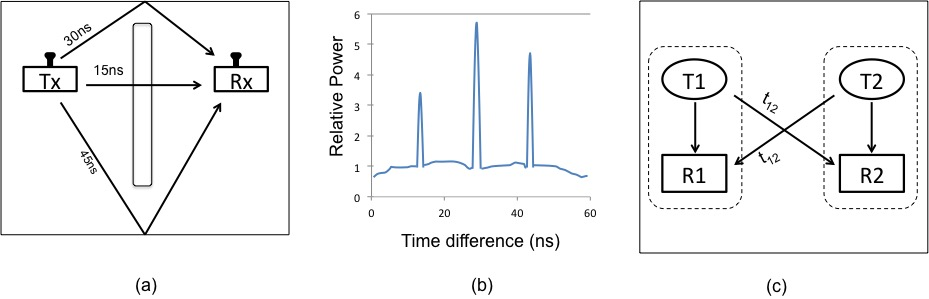
\includegraphics[width=0.9\textwidth]{figures/experiment.jpg}
\compactimg
\caption{(a) Depicts the wireless signal from a transmitter to receiver traversing there signal paths. (b) A plot of the relative signal power received corresponding to different times-of-flight. The first peak corresponds to the direct signal path. (c) Our localization framework leverages channel measurements at receivers that are co-located with the two LP-WAN clients to measure the relative time-of-flight between them: $t_{12}$.}
\label{fig:localize}
\end{figure*}

Our solution to overcome this challenge exploits the fact that LP-WAN radios, while being narrowband, regularly hop between a wide range of frequencies due to FCC mandated frequency-hopping. Our key idea is to stitch together wireless channel state information (CSI) measurements from these open frequencies to emulate a wide-band radio. Indeed, LP-WAN radios have a range of available frequencies to operate on -- including the 433~MHz, 900~MHz and whitespace frequencies (several bands in the 450-700 MHz range), together spanning a very wide bandwidth. Channel State Information obtained from these frequencies can then be processed to obtain time of flight at  a significantly higher resolution -- a few meters. Our solution builds upon recent work to combine channel information across frequencies in the WiFi context~\cite{vasisht2016decimeter}, while accounting for properties unique to LP-WANs such as power-constraints, hardware imperfections and limited receive-capability of LP-WAN hardware. 

To demonstrate our approach, mathematically, consider a signal that experiences a time-of-flight $\tau_{12}$ when traversing from a transmitter-1 to receiver-2 along line-of-sight. We assume that the transmitter and receiver operate on identical frequencies and are synchronized in time and phase (we consider hardware non-idealities in Sec.~\ref{sec:nonideal}). We can write the wireless channel experienced by this signal at any frequency $f$ as:
\begin{align}
h_f = A e^{-j 2 \pi f \tau_{12}}
\end{align}

where $A$ is signal the amplitude. %The phase of the channel is thus:
%
%\begin{align}
%\angle h_f = -j 2 \pi f %\tau_{12}~~\mod 2\pi %\label{eqn:channelphase}
%\end{align}
%
Solving for $\tau_{12}$, we find
%
\begin{align}
\tau_{12} = -\angle h_f /{(2 \pi f)}~~~\mod	1/f	\label{eqn:channelphase}
\end{align}
%
Note that the above equation computes time-of-flight modulo $1/f$. By hopping across a range of frequencies, one would obtain the time-of-flight with different modulo values. By combining these equations (using the Chinese Remainder Theorem~\cite{vasisht2016decimeter, ding1996chinese}), one can compute the time-of-flight with high resolution. We note that the above approach can be readily extended to settings where signals traverse more than one path, by combining measurements across frequencies.  Here, one can apply standard signal processing algorithms such as Bartlett~\cite{kumar2014accurate} or MUSIC~\cite{xiong2013arraytrack} to estimate the power of the signals along paths corresponding to different times-of-flight:
\begin{align}
P(\tau) = \left|\sum_f h_f e^{2 \pi f \tau}\right|^2 \label{eqn:ptau}
\end{align}
Fig.~\ref{fig:localize}(b) depicts this profile computed for a simple example of signals traversing along three paths as shown in Fig.~\ref{fig:localize}(a). Of the three paths, the direct path is the shortest and corresponds to the least time-of-flight. Hence, we can compute distance between the two devices by simply identifying the first peak in $P(\tau)$.

We note that the above approach requires measuring wireless channel state information on client devices. However, building a low-energy mechanism to do so on commodity LP-WAN devices is challenging. Indeed commodity radios from LoRa and SIGFOX are employ simple receive chains that are not designed to provide low-level signal information~\cite{alliance2015lorawan, zuniga2016sigfox}.

%\bob{SigFox implements a downlink, and it is described in the referenced IETF document.  Network practices severely limit the number of daily downlink messages per day (four).  Weightless-N was originally a one-way scheme.  Weightless-P tries to fix that.  The real limitation on Class A LoRa downlink messages is that they have to be queued and are dependent on the device initiating a transmit-receive sequence.} 

To resolve this challenge, we advocate augmenting some LP-WAN clients that have available wall-power, with low-cost receivers that are capable of obtaining channel state information. These radios can then be co-located with a subset of transmitting devices and record wireless channels from the base station and nearby devices. Given that these devices need to only measure CSI and not perform full-scale decoding, we can implement them using cheap off-the-shelf hardware. Our proof-of-concept implementation in Sec.~\ref{sec:eval} considers a subset of LP-WAN clients equipped with low-cost ($\sim$ \$10) RTL-SDR software radios~\cite{rtlsdr}.\footnote{We believe future designs can incorporate low-power CC1200 radios that provide channel state information, while drawing only 0.5$\mu$A of current when idle.} In this scenario, one must still  localize battery-powered client devices that do not have sophisticated receive chains -- a challenge we overcome in Sec.~\ref{sec:localization-inter}.

 

\subsection{Hardware Non-Idealities}\label{sec:nonideal}

Our discussion thus far has ignored a critical challenge faced by low-cost transmitters and receivers -- their hardware non-idealities. Specifically, low-power radios are driven by inexpensive oscillators that tend to drift over time. This drift creates three different offsets in the channel state-information gathered between low-power client devices: (1) A Frequency Offset: Stemming from the fact that the transmitter and receiver may operate at slightly different center frequencies; (2) A Timing Offset: The receiver may detect the transmitted signal at an arbitrary delay, which affects the measured channel state information; (3) A Phase Offset: A random phase error introduced to the CSI whenever the hardware restarts, introduced by the Phase Locked Loop (PLL) of the transmitter and receiver. 

Mathematically, these three offsets have a direct impact on the phase of the wireless channel. In particular, we can re-write Eqn.~\ref{eqn:channelphase} of the wireless channel captured at time $t$ to incorporate offsets in time $\Delta t$, frequency $\Delta f$ and phase $\Delta \phi$ as follows:
\begin{align}
\angle h_f = -j~(2 \pi f \tau_{12} + 2 \pi \Delta f t + 2 \pi f \Delta \tau + \Delta \phi) ~~\mod 2\pi
\end{align}

Complicating matters further is the fact that our nodes have two radios each -- one to transmit and one to receive channel state information, each driven by different clocks. This implies that we get four unique values for each offset, one between every transmitter-receiver pair within and across client nodes.

We overcome this challenge by exploiting the structure of  frequency offsets. Specifically, we leverage the fact that given that transmitters and receivers are co-located, their relative time-of-flight is known a priori. As a result, one can use estimates of the channel between the co-located transmitter-receiver pair at each client node to remove the offsets between two nodes. 

To illustrate our approach mathematically, let's consider the configuration shown in Fig.~\ref{fig:localize}(c).  Here, the sender $T_1$ with time delay $\Delta t_1$, frequency $f_1$, phase $\phi_1$, transmits a signal received with time delay $\Delta t_2$, frequency $f_2$, phase $\phi_2$ by $R_2$. We can then write the wireless channel between transmitter $T_1$ and receiver $R_2$ as:
\begin{align}
\angle h_{T_1 \rightarrow R_2} = -j~(2 \pi f_{R_2} \tau_{12} + 2 \pi (f_{T_1} - f_{R_2}) t\hspace*{2cm} \nonumber \\
+ 2 \pi f (\Delta t_{T_1} + \Delta t_{R_2}) +(\phi_{T_1} - \phi_{R_2}) ) ~~\mod 2\pi \label{eqn:h1}
\end{align}
One can then write similar equations for channels between every transmitter, receiver pair. However,  note two properties: First, the time-of-flight and delays between co-located transmitter, receiver pairs is constant -- and can therefore be calibrated a-priori. Without loss of generality, we can assume the time-of-flight is zero to write:
\begin{align}
\angle h_{T_1 \rightarrow R_1} = -j~(2 \pi (f_{T_1} - f_{R_1}) t + 2 \pi f (\Delta t_{T_1} + \Delta t_{R_1})  \nonumber \\
+~(\phi_{T_1} - \phi_{R_1}) ) ~~\mod 2\pi \label{eqn:h22}
\end{align}
Second, the time-of-flight experienced by signals from the transmitter to receiver and vice-versa are identical. 
%In other words, we can write the channels from $T_2$ to $R_1$ as:
%\begin{align}
%\angle h_{T_2 \rightarrow R_1} =&  -j~(2 \pi f_{R_1} \tau_{12} + 2 \pi (f_{T_2} - f_{R_1}) t   \nonumber \\
%& + 2 \pi f (\Delta t_{T_2} + \Delta t_{R_1}) +~(\phi_{T_2} - \phi_{R_1}) ) ~~\mod 2\pi \label{eqn:h3}
%\end{align}
Combining Eqn.\ref{eqn:h1}-\ref{eqn:h22}:
\begin{align}
\angle \left(\frac{h_{T_1 \rightarrow R_2} h_{T_2 \rightarrow R_1}}{h_{T_1 \rightarrow R_1} h_{T_2 \rightarrow R_2}} \right) = -j~4 \pi f_{R_1} \tau_{12} ~~\mod 2\pi \label{eqn:h4}
\end{align}
Therefore,  $\hat{h}_f = \frac{h_{T_1 \rightarrow R_2} h_{T_2 \rightarrow R_1}}{h_{T_1 \rightarrow R_1} h_{T_2 \rightarrow R_2}}$ is independent of frequency offsets. Hence, we can rewrite Eqn.~\ref{eqn:ptau} using the modified channels, to measure time-of-flight in the presence of multiple signal paths as:
\begin{align}
P(\tau) = \left|\sum_f \frac{h_{T_1 \rightarrow R_2} h_{T_2 \rightarrow R_1}}{h_{T_1 \rightarrow R_1} h_{T_2 \rightarrow R_2}} e^{4 \pi f \tau}\right|^2 =  \left|\sum_f \hat{h}_f e^{4 \pi f \tau}\right|^2\label{eqn:ptau2}
\end{align}

Thus, we can estimate time-of-flight between two clients, despite the two radios on each experiencing arbitrary hardware offsets. 


\subsection{Finding Absolute Localization}\label{sec:localization-abs}
Given relative locations as calculated from pairwise times-of-flight, one would still need to find the absolute location of client nodes. We must do so solely using given pairwise distances between several pairs of nodes -- some of which at known absolute locations (e.g. the base stations themselves). However, our approach should also deal with uncertainty in observed distances, owing to  noise. 

We propose to exploit the extensive past work on network localization to overcome this problem. Past work has shown how one can model the wireless network topology as a graph with pair-wise distances between sensor nodes along with their uncertainties labeled as edge weights~\cite{nwlocalization}. Assuming that the graph is rigid, one can then use the known location of a subset of these nodes to calculate the location of the remaining nodes~\cite{sethnwlocalization}.


\subsection{Locating Battery-Powered Devices and Sources of Interference}\label{sec:localization-inter}

This section extends our localization framework to devices where channel state information is not available. For instance, consider battery-powered LP-WAN nodes whose RF-chains are not sophisticated enough to measure channel state information. Or consider interferers transmitting on the same frequencies, whose channel state information is not available to the network. Our approach to locate these devices leverages the availability of nearby powered clients that can measure signals from these nodes. However, a crucial challenge when dealing with interfering sources, in particular, is that their channels cannot also be measured at our own powered clients, given that the signals interferers transmit are potentially unknown. In other words, we would need to locate  interferers without knowledge of their transmitted signals or any cooperation. 

We address this challenge by measuring time-difference of arrival, as opposed to time-of-arrival between a transmitting source and two powered clients that listen to the node of interest. Specifically, for each transmitter $I$, we capture the wireless signal $y_{I->R_1}$ and $y_{I->R_2}$ measured by the receive chains of our two clients. One can then write these received signal as a function of the potentially unknown transmitted signal $x_I$, and  corresponding channels as: 
\begin{align*}
y_{I->R_1} =  h_{I->R_1} x_I \text{~~and~~} y_{I->R_2} = h_{I->R_2} x_I 
\end{align*}

It is then easy to see that $y_{I->R_1}/y_{I->R_1}$ is a function independent of the transmitted signal and depends purely on the wireless channels from the transmitter to the receive chains. More specifically, it depends on the time-difference of arrival between the transmitter to either receiver. However, like before, it is once again subject to time, frequency and phase offsets. Interestingly, the time-difference of arrival can be written purely in terms of the hardware non-idealities of our own powered clients. To see how, observe that: 
\begin{align*}
\angle y_{I \rightarrow R_1} /  y_{I \rightarrow R_2} = & -j~(2 \pi f_{R_2} (\tau_{I \rightarrow R_1} - \tau_{I \rightarrow R_2}) + 2 \pi (f_{R_1} - f_{R_2}) t \nonumber \\
& + 2 \pi f_{R_2} (\Delta t_{R_1} - \Delta t_{R_2})  +~(\phi_{R_1} - \phi_{R_2}) ) \mod 2\pi \label{eqn:h2}
\end{align*}

Let's assume that at the same time $t$ we have a packet sent from one of the transmit chains of our powered clients to the two receivers, we can then write:
\begin{align*}
\angle h_{T_1 \rightarrow R_1} /  h_{T_1 \rightarrow R_2} = & -j~(- 2 \pi f_{R_2}\tau_{12} + 2 \pi (f_{R_1} - f_{R_2}) t \nonumber \\
& + 2 \pi f_{R_2} (\Delta t_{R_1} - \Delta t_{R_2})  +~(\phi_{R_1} - \phi_{R_2}) ) \mod 2\pi 
\end{align*}

Combining the above two equations, we observe that the quantity $\frac{y_{I \rightarrow R_1} h_{T_1 \rightarrow R_2}}{y_{I \rightarrow R_2} h_{T_1 \rightarrow R_1}}$ is independent of hardware offset as well as the transmitted signal of $I$ and depends purely on the time-difference of arrival $\tau_{I \rightarrow R_1} - \tau_{I \rightarrow R_2}$, as well as the known time-of-flight $\tau_{12}$ between our two powered sensor clients. Consequently, we can measure the time-difference-of-arrival by extending Eqn.~\ref{eqn:ptau2} as:
\begin{align}
P(\tau) = \left|\sum_f \frac{y_{I \rightarrow R_1} h_{T_1 \rightarrow R_2}}{y_{I \rightarrow R_2} h_{T_1 \rightarrow R_1}} e^{4 \pi f (\tau + \tau_{12}) }\right|^2 
\end{align}
By computing the time-differences between  $I$ and three or more powered clients, one can obtain its location relative to them. Given that the absolute location of powered clients can be obtained using the algorithms in Sec.~\ref{sec:localization-abs}, one can obtain the absolute position of  interfering and battery-powered sources as well.

\section{Implementation}
\label{sec:arch}

{\color{red} This section is relevant but needs major revisioning!}

% \begin{figure*}[!hbt]
% \centering
% 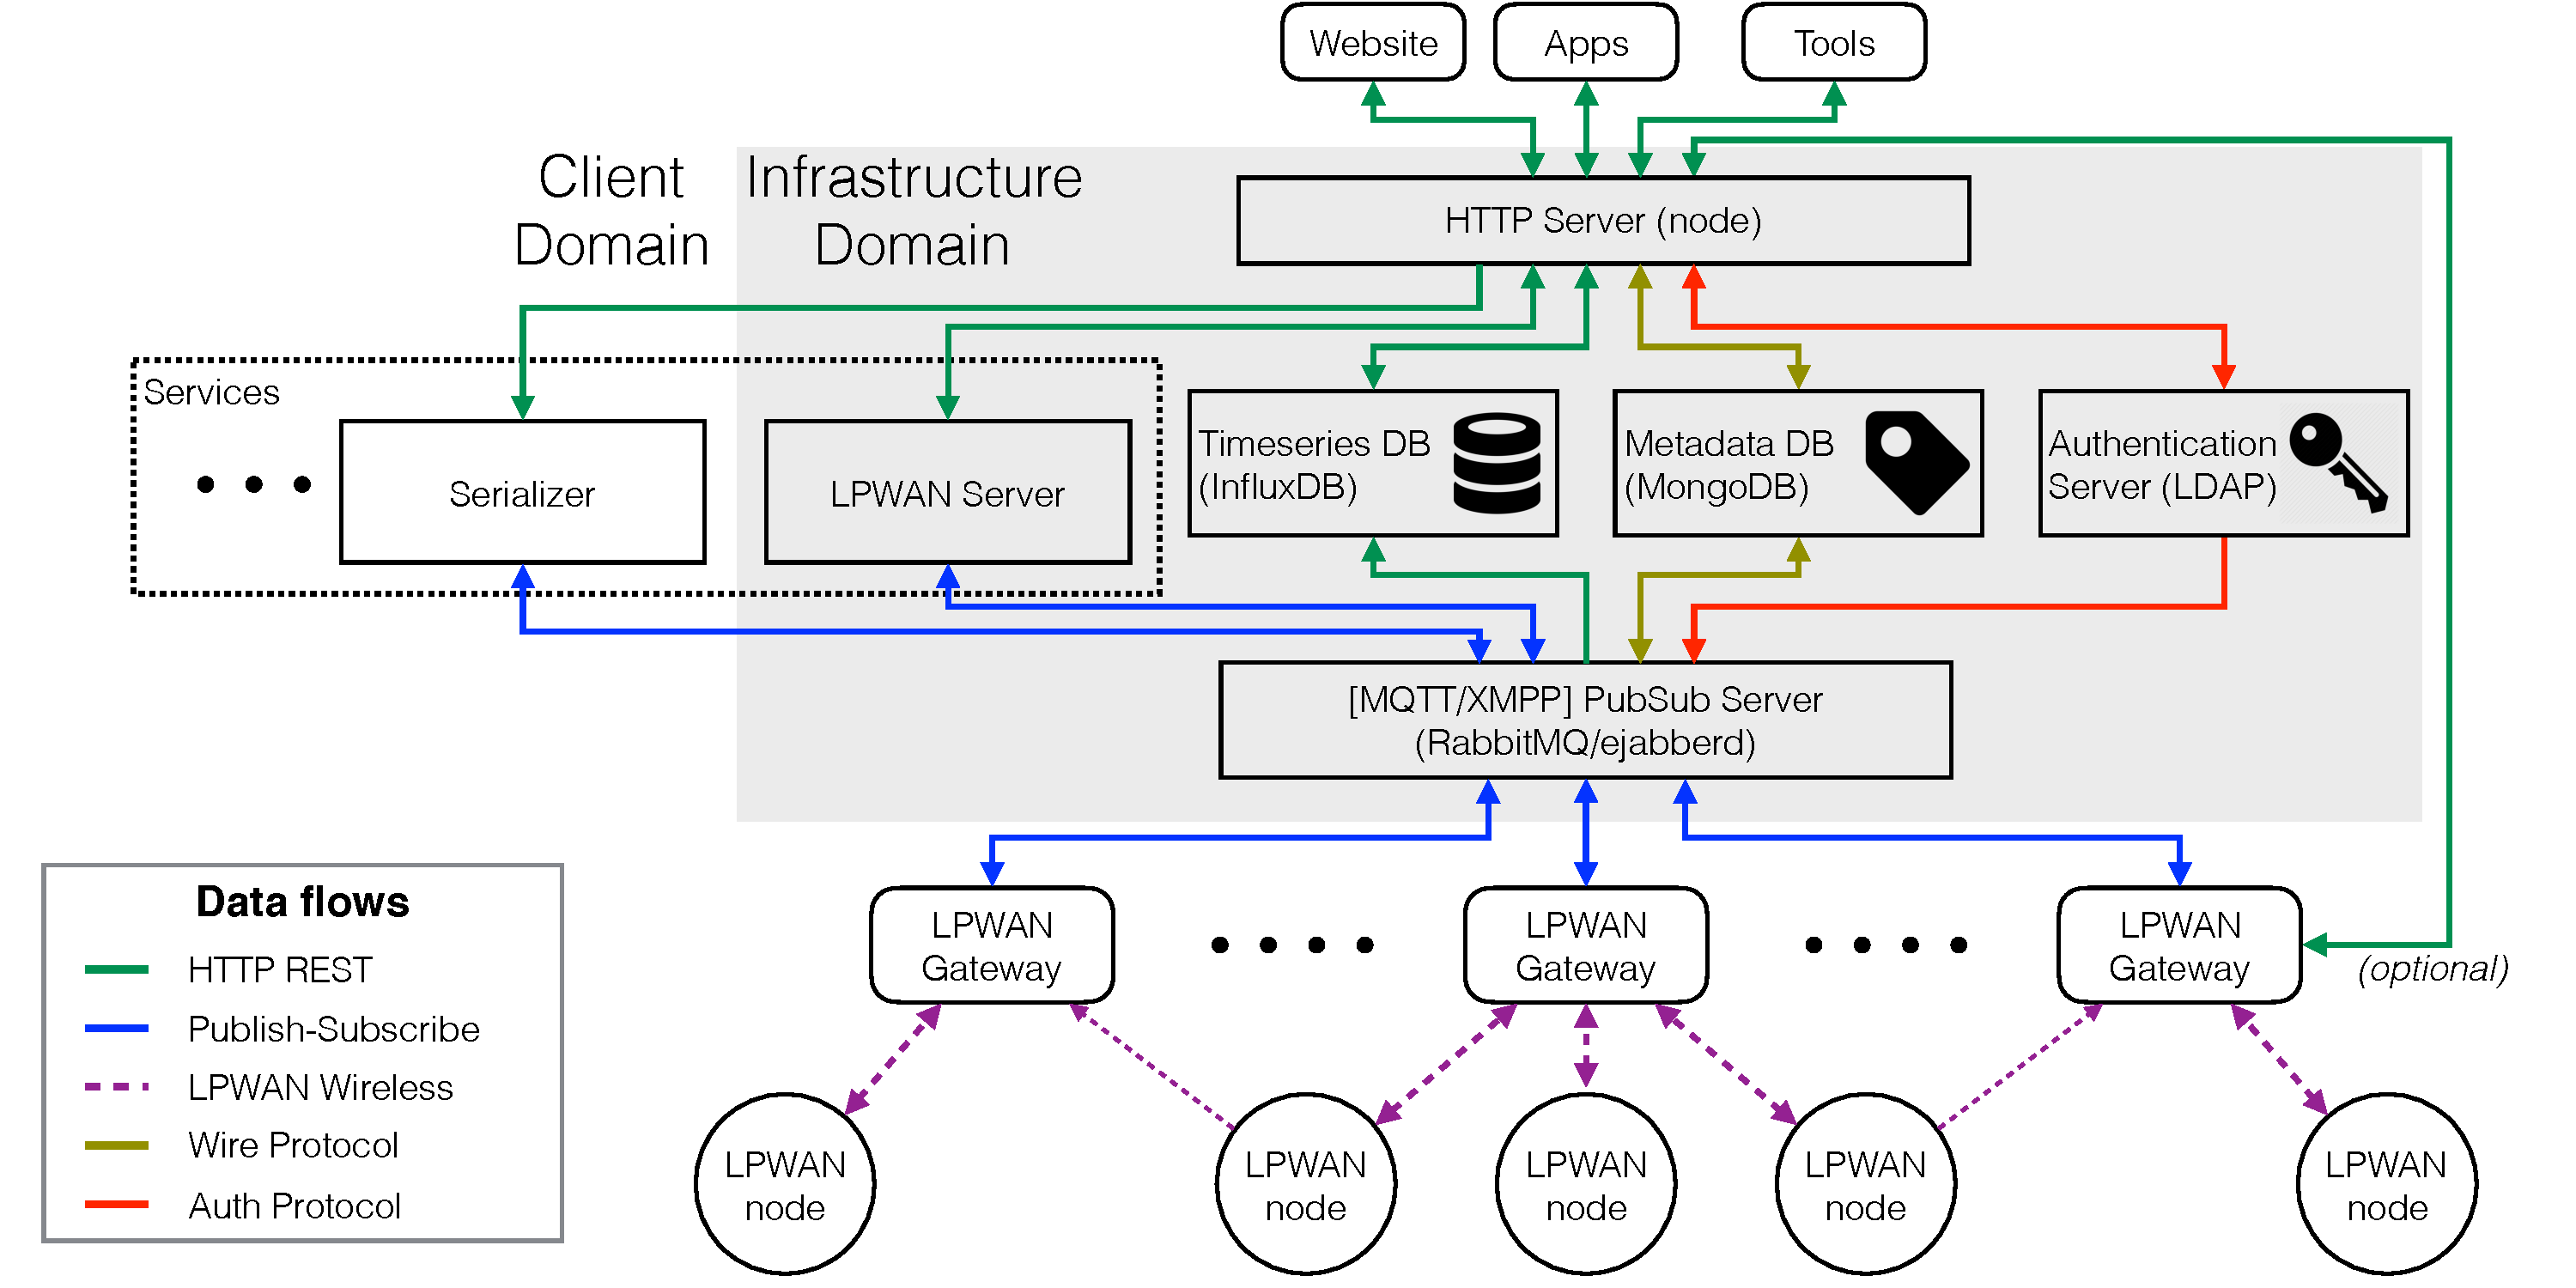
\includegraphics[width=0.6\textwidth]{figures/openChirp_architecture}
% \compactimg
% \caption{System Architecture}
% \label{fig:openchirp-arch}
% \end{figure*}


\begin{figure}%[!ht]
\centering
\compactimg
\subfloat{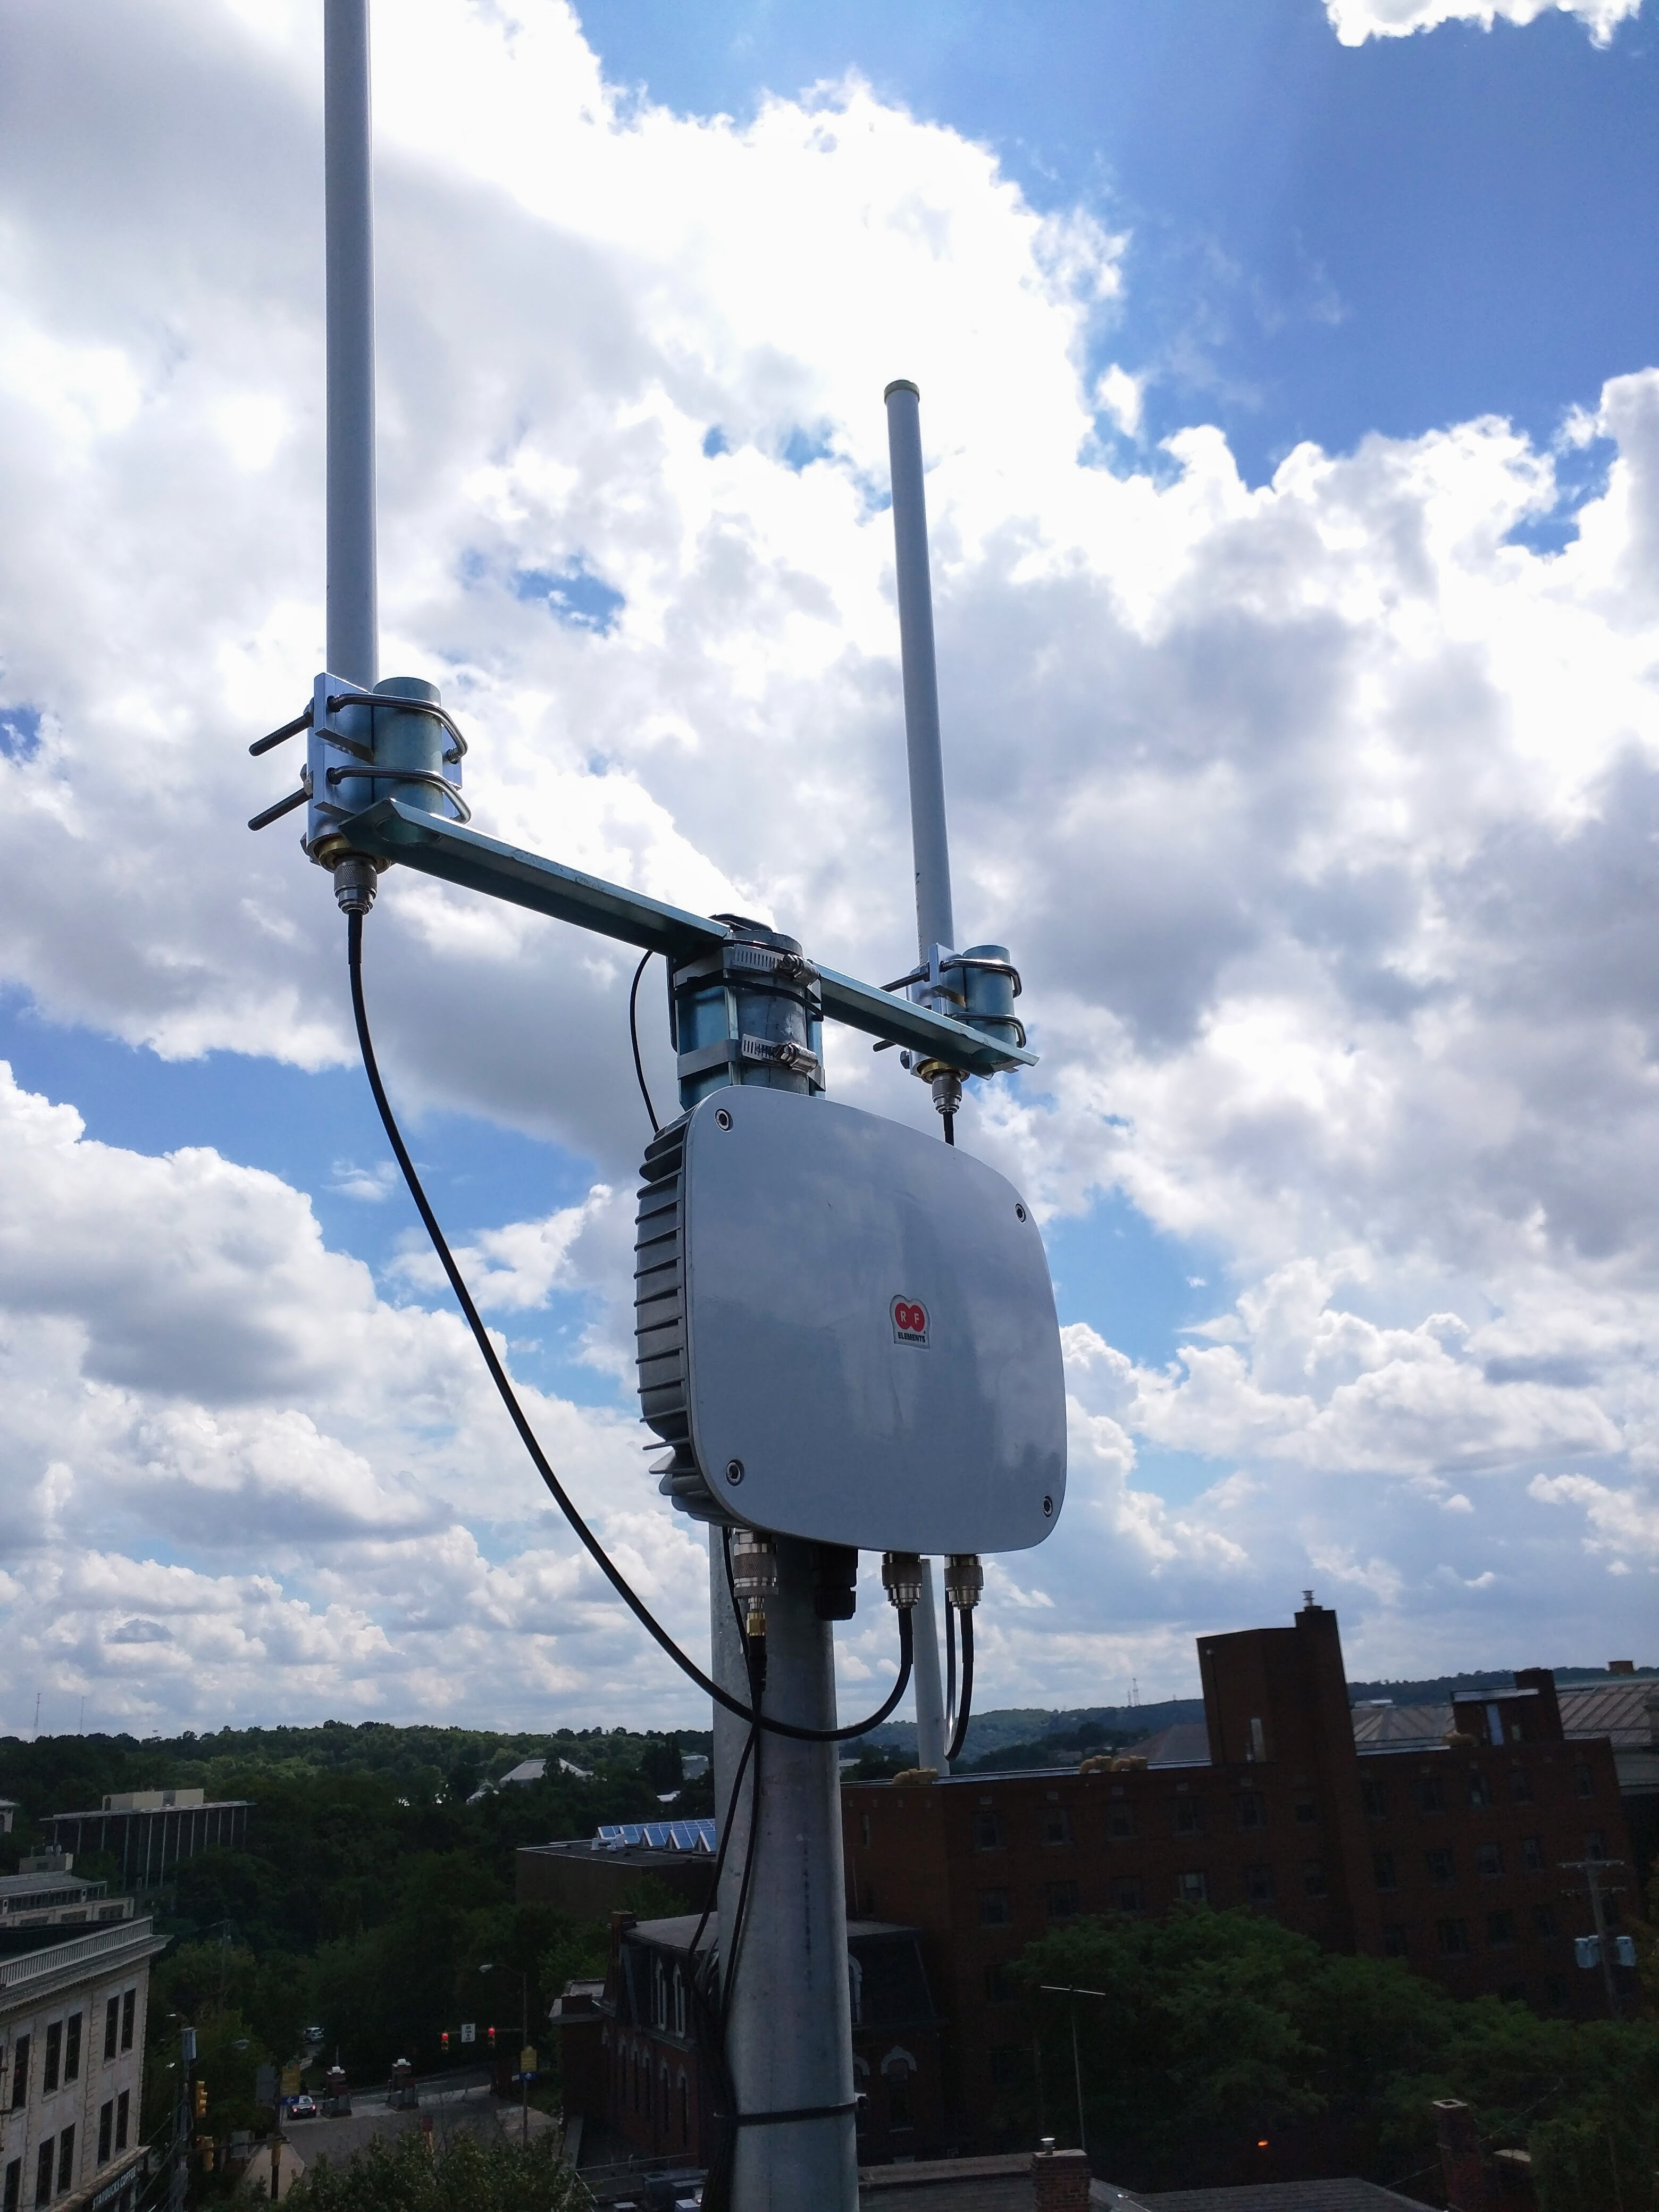
\includegraphics[height=3.9cm]{figures/gateway_deployment.jpeg}
\label{fig:gateway-photo}}
\hfill
\subfloat{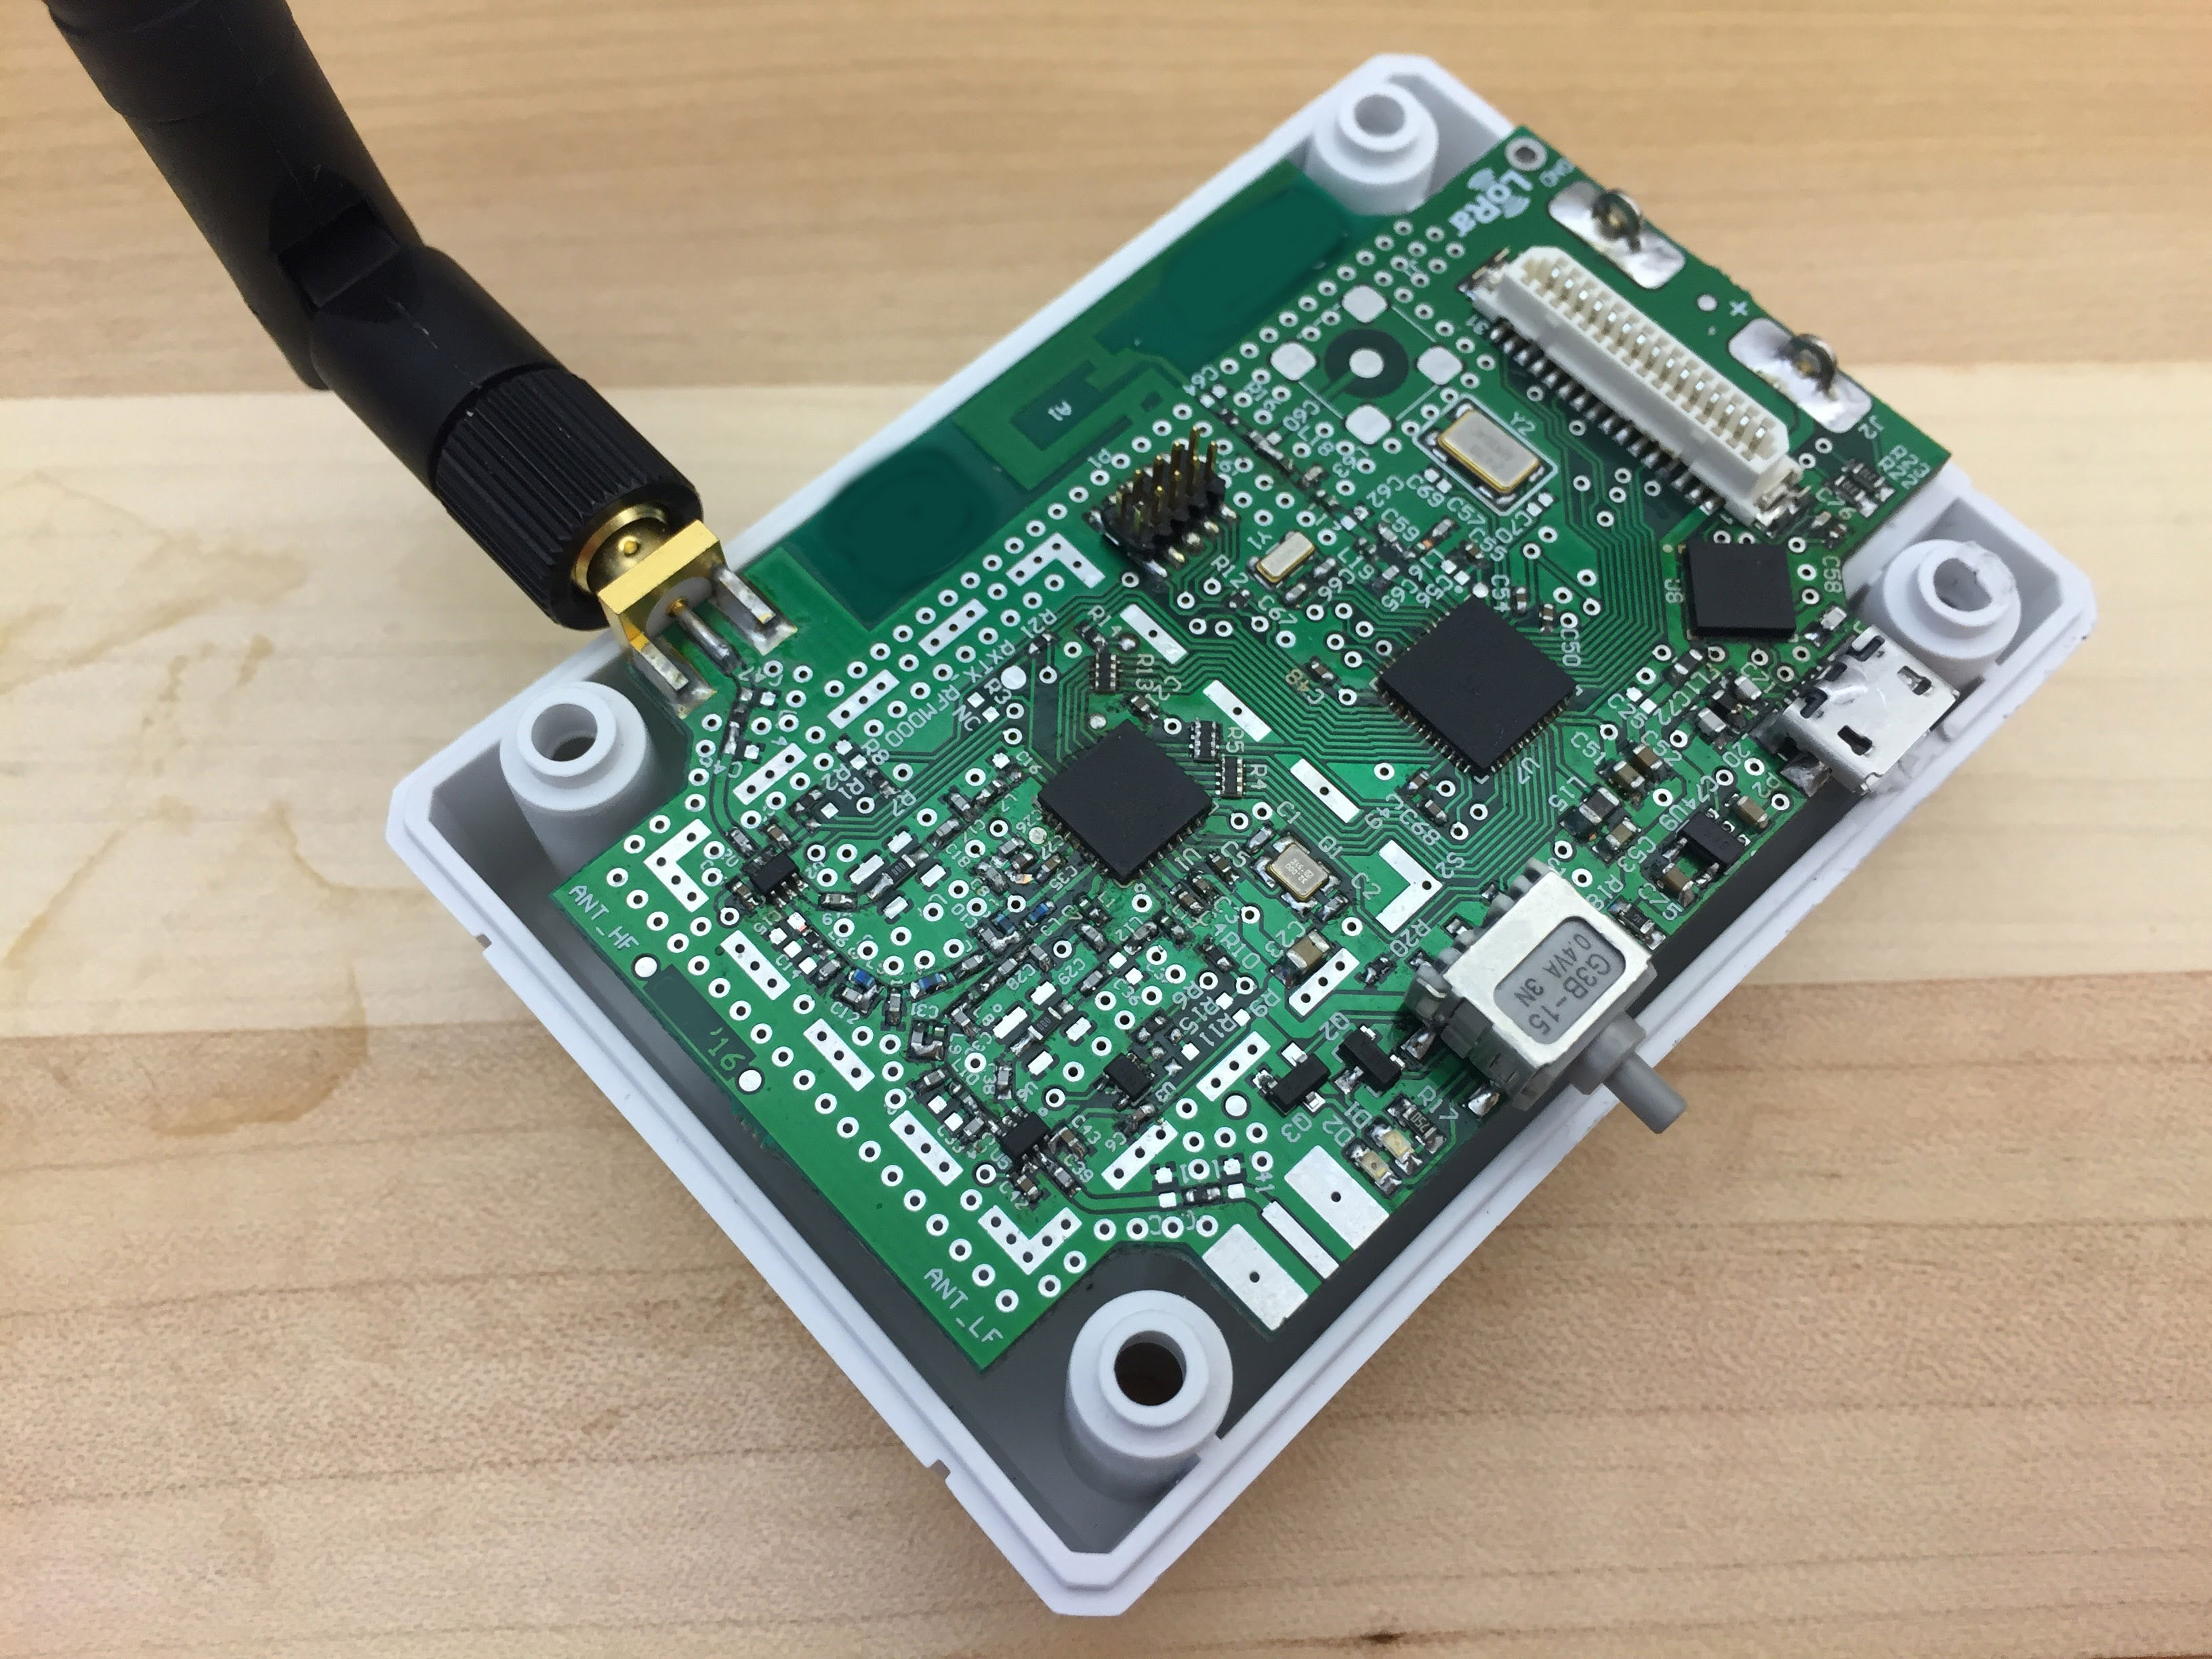
\includegraphics[height=3.9cm]{figures/receiver_anon.jpg}
\label{fig:lorabug-photo}}
\caption{Photo of our gateway (left) and a custom client node (right)}
\end{figure}



We implemented and evaluated our system extensively both through proof-of-concept experiments and trace-driven simulations to evaluate performance at scale. Our simulations were performed using traces gathered through a university campus-scale deployment of LoRaWAN base stations. We describe our hardware, testbed, measurements gathered, simulations and experiments below. 

%In the purest sense, a LoRaWAN server is responsible for delivering binary data blobs to and from an application.  To meet the needs of future multi-tenant city-scale sensing applications, we designed the OpenChirp which builds on top of LoRaWAN by adding a user management framework, application interface and a set of core services for performing data serialization (converting over-the-air binary data into a typed form with a schema), meta-data management and time series data storage.  

\vspace*{0.1cm}\noindent \textbf{Infrastructure Software Architecture: } {\color{blue} Add a description of the OC architecture. Refer to website for the problems it solves...}

\vspace*{0.1cm}\noindent \textbf{Base Station Hardware: } Our pilot deployment gateways used a standard single concentrator chipset that is able to receive on 8-channels simultaneously. Though ideal for low-cost deployments like what a user might deploy in their home, this does not exploit the entire LoRa spectrum.  For this purpose, we developed a more capable second-generation gateway, shown in \figref{64-chan-gw} that is able to operate on all 64-channels simultaneously. 
Similar to the 8-channel gateway, the 64 channel gateway is controlled by a single Raspberry Pi 3. Eight LoRa concentrator cards are used to interact simultaneously with 64 125kHz and 8 500kHz uplink (receive) channels and 8 500kHz downlink (transmit) channels. This spans the complete US LoRaWAN specified channel list from 902.3 to 914.9MHz for uplink and 923.3 to 927.5MHz for downlink. The radio cards are stacked in rows of four to optimize space inside the gateway enclosure. A Ublox GPS timing module is onboard to supply precise timestamps for incoming packets, synchronize time slots in LoRaWAN Class B, and to localize the gateways in the network. For future research, the board-to-board interface facilitates board stacks past that of dual 4 radio boards, while maintaining only a single USB connection to the Raspberry Pi host. This allows the radio board stack to be used with more powerful or generic machines that may not have GPIO and SPI peripherals. Additionally, the radio cards are secured into PCI Express Mini connector that expose many common wire protocols, which ensures upgradeability. We include an RTL software-defined radio for sensing of white spaces and listen-before-talk (LBT) functionality. For extended use in rough outdoor environments, we hardened the deployed hardware (weather-resistant design) and software (watchdog resets). The gateway is fully network connected and power using Power-Over-Ethernet(POE). \figref{gateway-photo} shows one of our four pilot rooftop gateways.


% \begin{figure}%[!htb]
% \centering
% 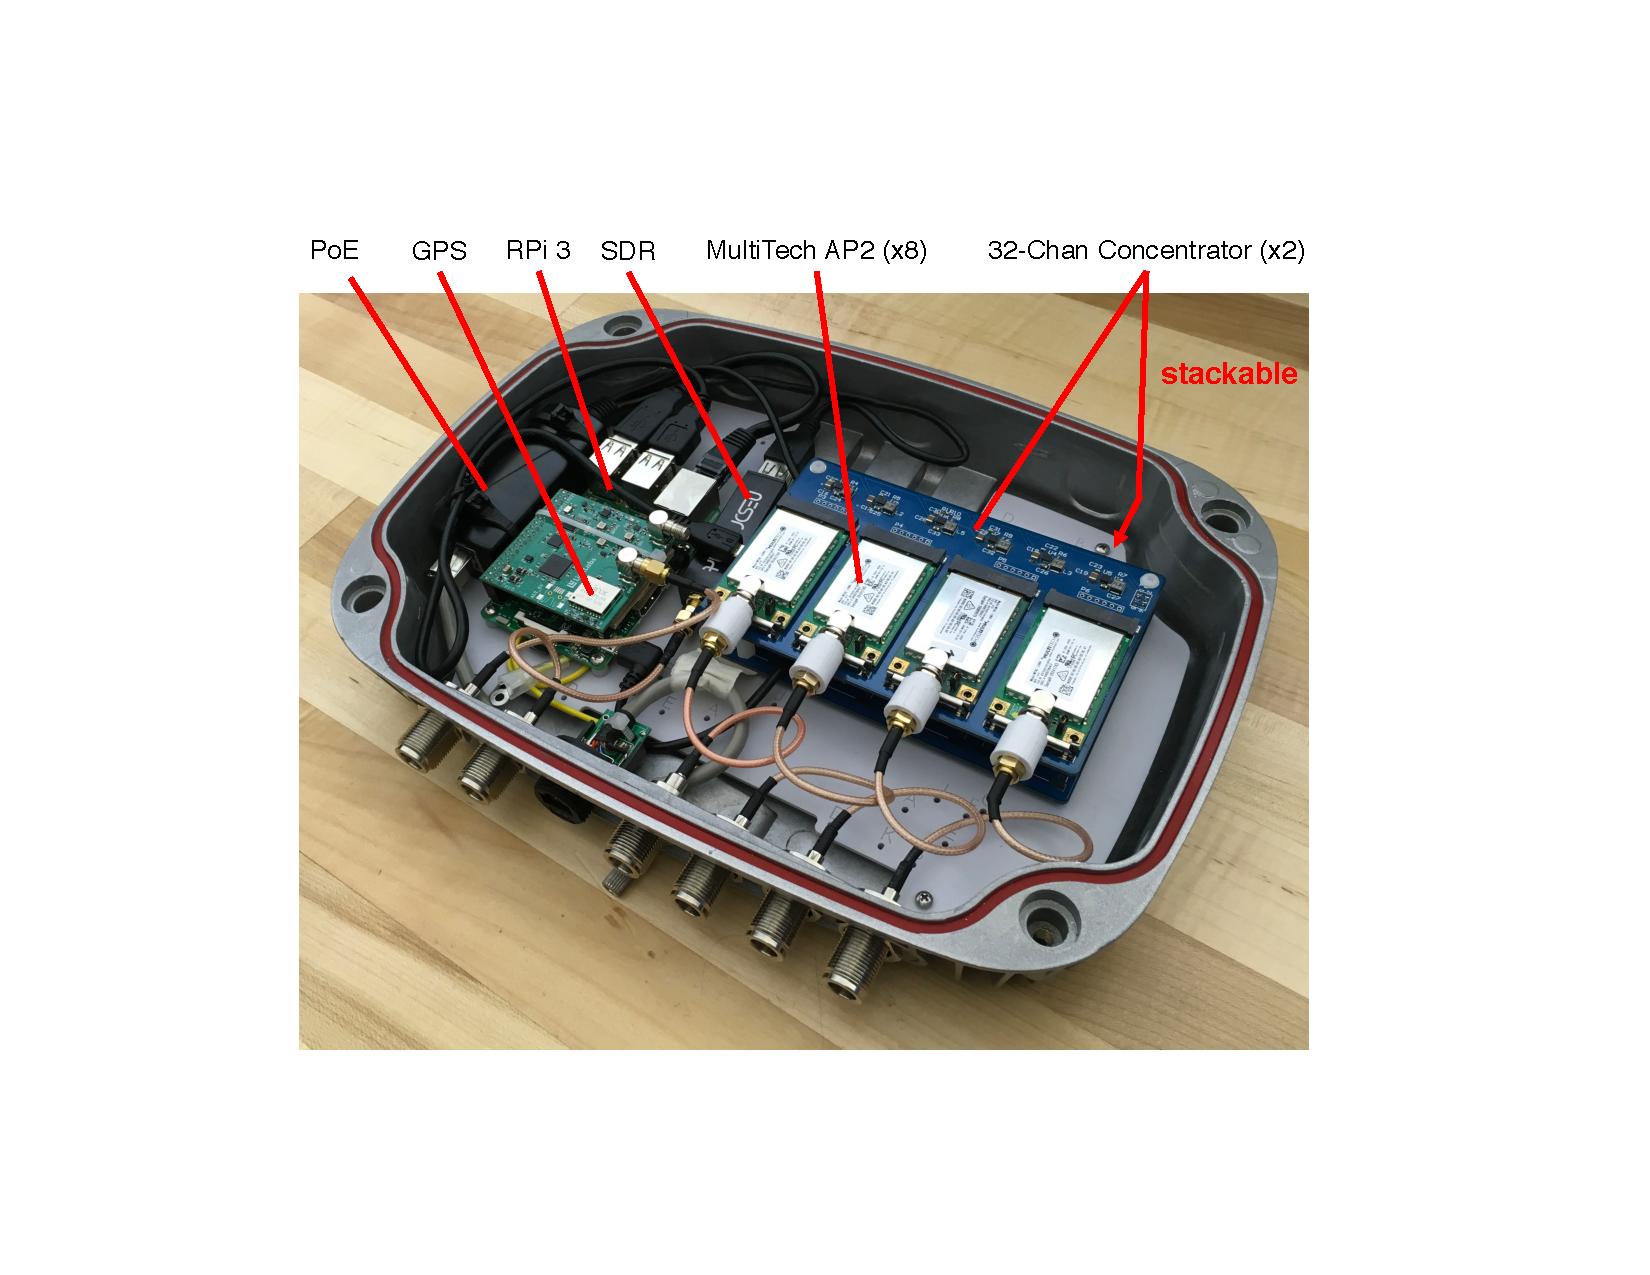
\includegraphics[width=0.4\textwidth]{figures/64-chan-photo.pdf}
% \compactimg
% \caption{Custom 64-channel gateway}
% \label{fig:64-chan-gw}
% \end{figure}

\begin{figure}%[!b]
\centering
%\compactimg
\compactimg
{\renewcommand{\arraystretch}{0}
\begin{tabular}{@{}c@{}}	
\subfloat{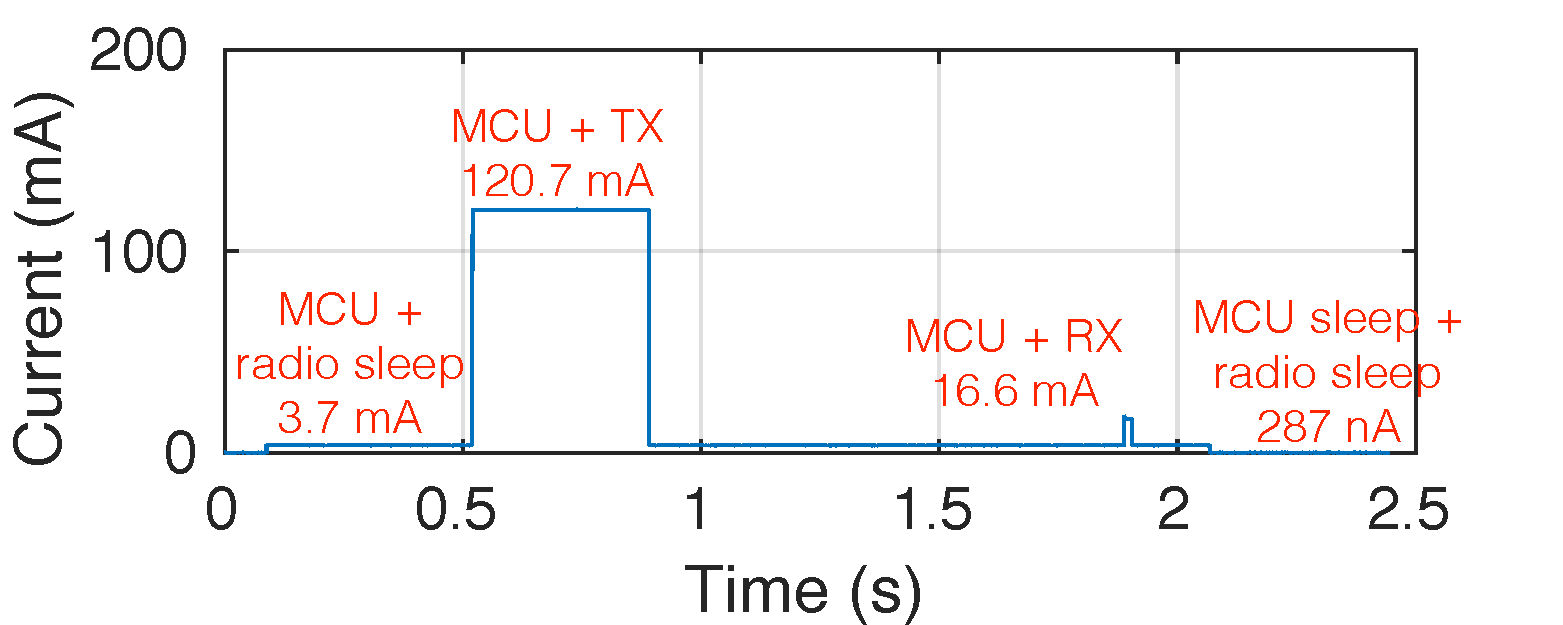
\includegraphics[width=0.4\textwidth]{figures/bug_power_trace_annotated} % NOTE: keep the \compactimg inside the subfloat comment to save space between the two images
\label{fig:power-trace}
} \\
\subfloat{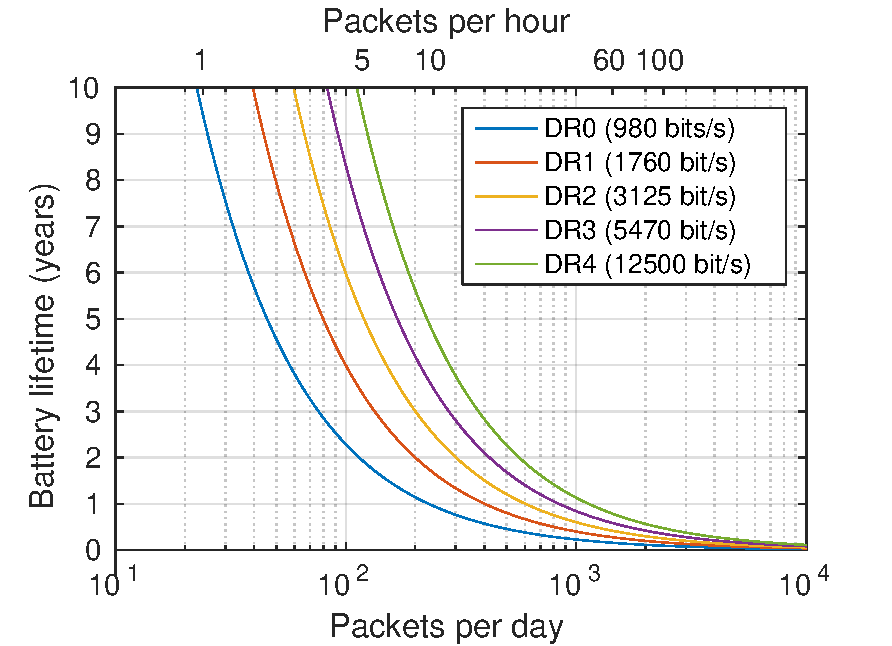
\includegraphics[width=0.4\textwidth]{figures/LoRaBug_AA_lifetime_semilog}
\label{fig:lifetime-estimates}
\compactimg}
\end{tabular}}
% \compactimg
\caption{(above) Custom LoRa client current consumption over time for transmitting a packet and then checking for an ACK from the gateway. (below) Lifetime of a custom LoRa client powered by two AA batteries at various operating points based on a measured energy profile.}
\end{figure}

{\color{red} Most of the custom client arguments like other platforms lacking BLE are not relevant anymore}

\vspace*{0.1cm}\noindent {\bf Custom LoRa Client:}   We found that many existing LoRa client implementations were not aggressively able to power down peripherals and few lacked BLE support which is extremely valuable for device provisioning. For this reason, we developed an open-source, low-cost, low-power, and extensible LPWAN end-node hardware platform shown in \figref{lorabug-photo}. The custom client is powered by a Texas Instruments CC2650 microcontroller (MCU) with integrated 2.4 GHz IEEE 802.15.4 and Bluetooth Low-Energy (BLE) radios. It communicates to LoRa networks through a Semtech SX1276 LoRa radio. The node can be augmented with expansion modules for a variety of applications (e.g. environmental sensing, GPS localization and actuation). In addition to typical sleep states, the MCU has an ultra low-power sensor co-processor for sensor sampling and data aggregation, and a cryptographic accelerator that enhances the performance of security functions and reduces code-size. The custom client hardware is housed in a small plastic enclosure that accommodates two AA batteries. 

%\begin{figure}[!htb]
%\centering
%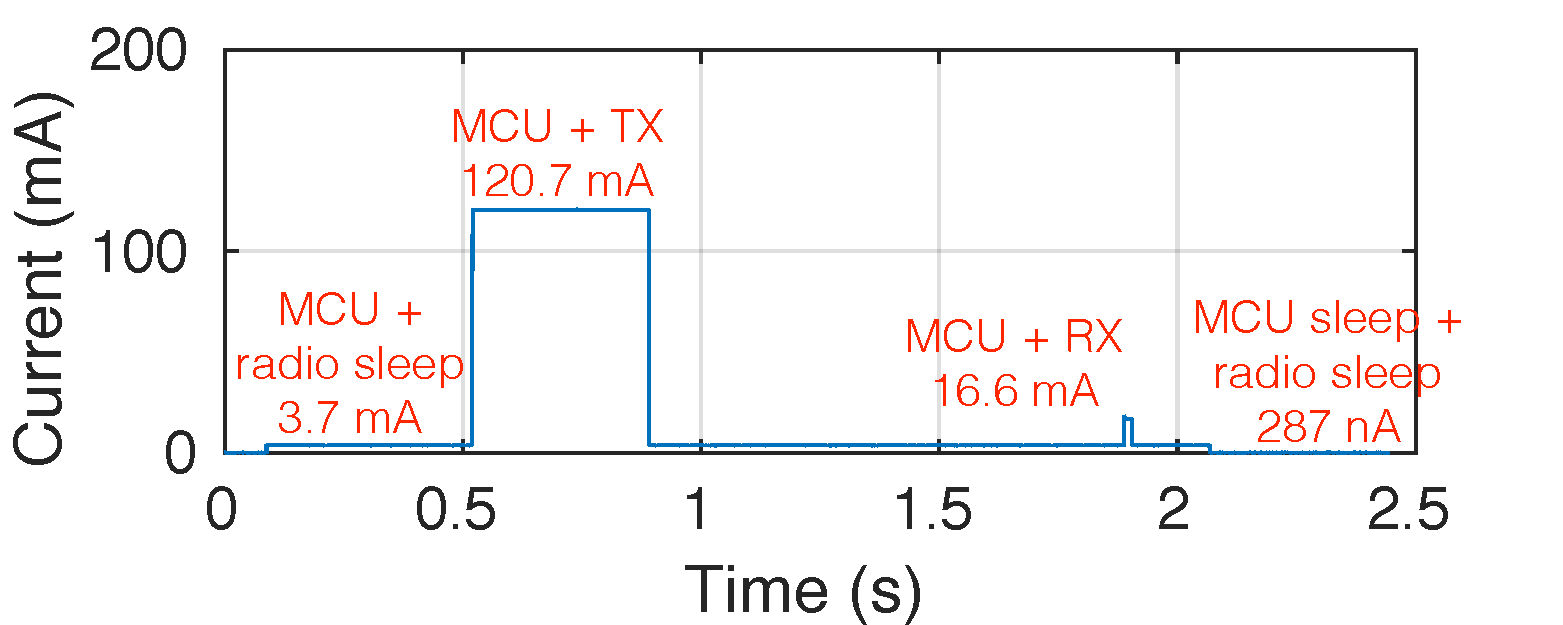
\includegraphics[width=0.4\textwidth]{figures/bug_power_trace_annotated.pdf}
%\compactimg
%\caption{{\color{blue} Add caption}}
%\label{fig:bug_power_trace}
%\end{figure}




Both our MCU and LoRa radio have multiple sleep and function states that consume varying amounts of power. In \figref{power-trace} we look at the current consumed by these devices while sending out 8 bytes of data and receiving an acknowledgment. The radio was configured for uplink communications with 125 kHz channel bandwidth, data rate of 980 bits/s, spreading factor of 10 and coding rate of $4/5$.  Based on a simple power model, we estimate the lifetime of these devices in \figref{lifetime-estimates} while operating on two 2000 mAH AA batteries (we make a conservative estimate of 60 \% usable energy and maximum shelf life of 10 years). Thus, with proper duty-cycling, the custom client can function and communicate for multiple years on simple batteries.





% \vspace*{0.1cm}\noindent{\bf Localization Testbed: } We conduct our localization experiments on a testbed composed of SX1276MB1LAS boards with an embedded LoRaWAN chip that
% is mBed compatible. We connect these boards with NUCLEO-L152RE boards with the mBed platform to program the LoRa chips to hop between a range of pre-specified frequencies. The boards operate at  center frequencies in the 433 MHz and 902 MHz ISM band over a bandwidth of 500~KHz or 125~KHz depending on the
% data rate the wireless channel supports~\cite{alliance2015lorawan}. We use the RTL-SDR~\cite{rtlsdr} platform to collect wireless channel measurements. The collected  wireless channels between transmitter-receiver pairs are aggregated at the base station, where they are processed using our C++/MATLAB based localization framework.










\section{Experimental Results}

\label{sec:eval}

% {\color{blue}
% [DIANA, ARTUR, ADWAIT, CRAIG]

% Evaluations are bottom-up
% \begin{itemize}
% \item Ranging performance (Experiment) (WITH FIGURE)
% \item New Link metrics (Experiment) (WITH FIGURE)
% \item Scale (Simulation) (WITH FIGURE)
% \item Coexistence (Simulation) (WITH FIGURE)
% \end{itemize}
% }

This section presents experimental results ans benchmarks used to drive large-scale simulations in \secref{simulations}

\subsection{LoRa Channel Model}

\begin{figure}%[!htb]
\centering
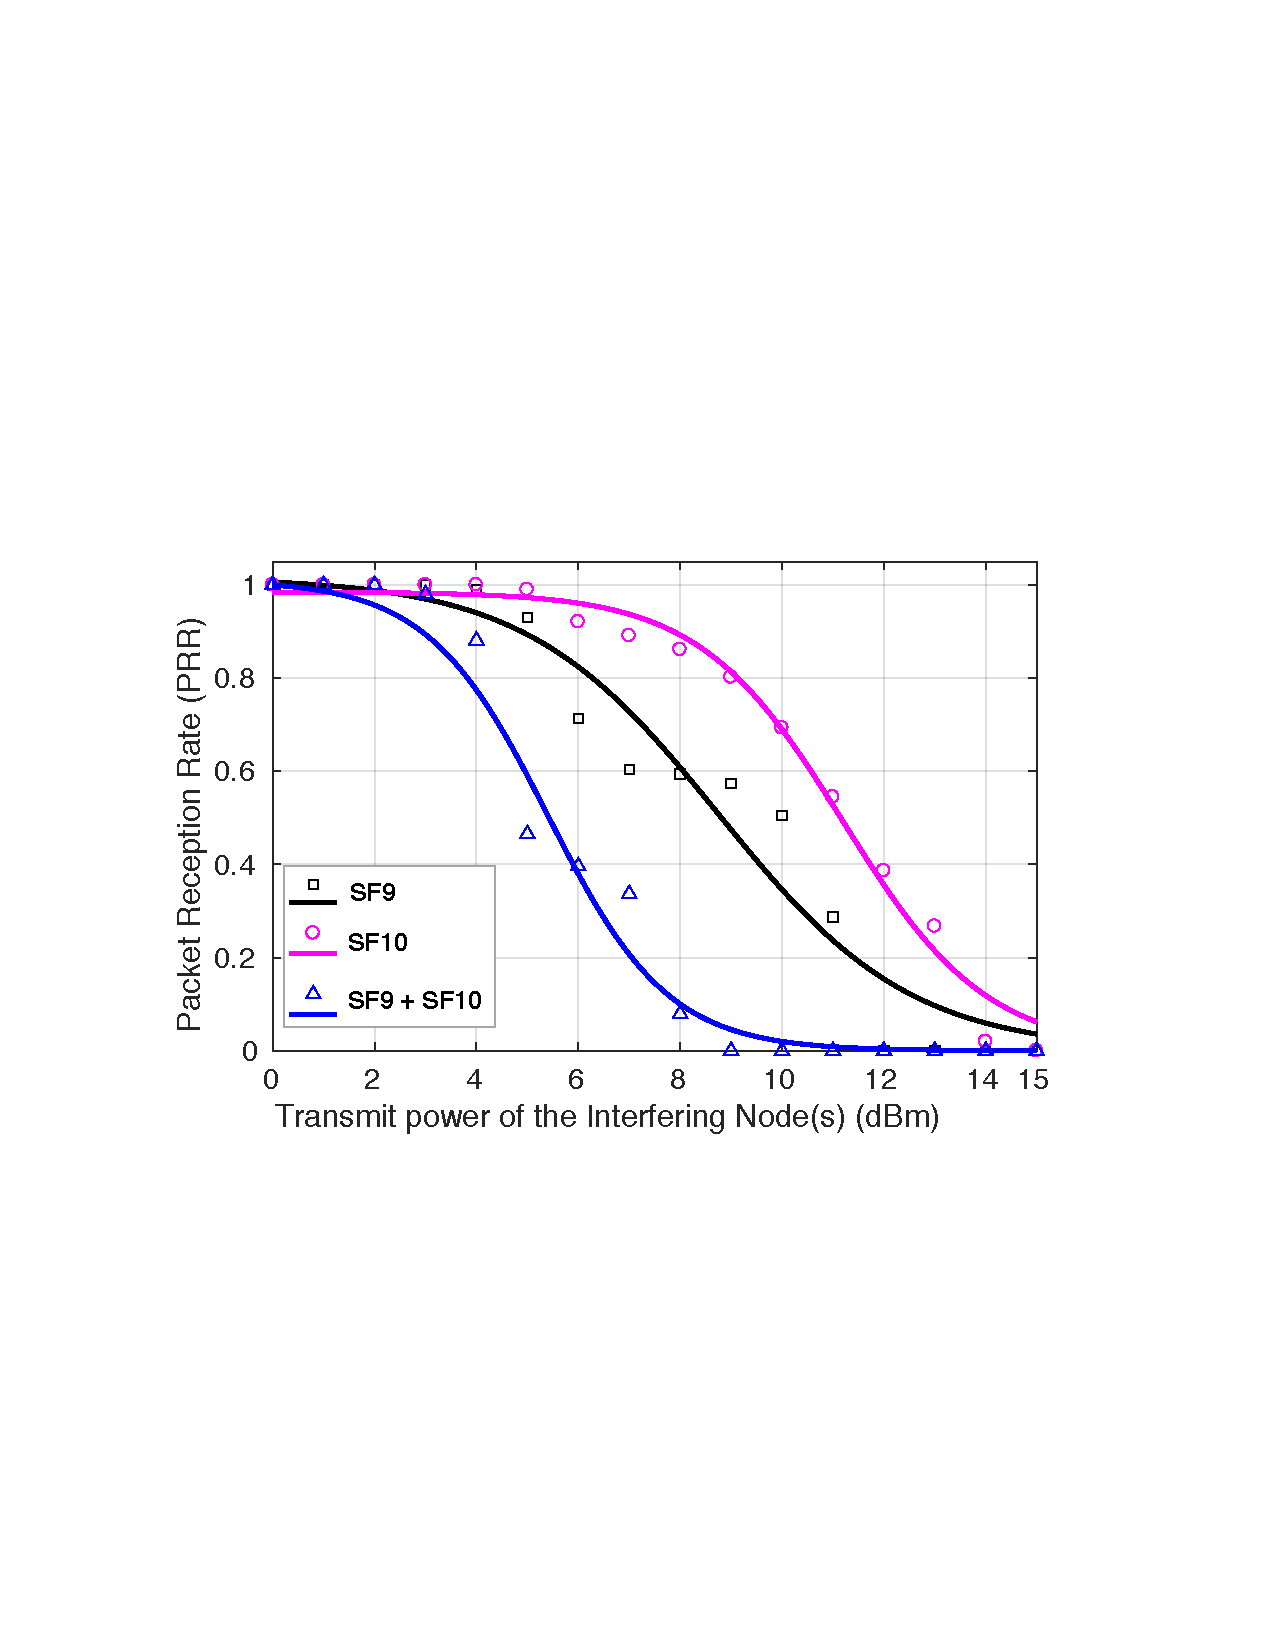
\includegraphics[width=0.8\columnwidth]{figures/aim-sf}
\compactimg
\caption{Packet Reception Rate (PRR) of packets sent at SF8 when overpowered by another transmission(s) on the same channel. We can also observe the additive interference caused by two simultaneous transmissions (SF9 and SF10).}
\label{fig:aim-sf}
\compactimg
\end{figure}

Our first experiment shows the interaction between different spreading factors as described by our additive interference model. Packets with varying configurations were sent out synchronously to force packet collisions and interference.
LoRa devices are calibrated for receive power and placed at a distance of 3 $m$ from the gateway. 

\figref{aim-sf} shows the packet reception rate of a node using spreading factor 8 (transmitting at 0 dBm) when sharing the same frequency with other node(s) using: spreading factor 9, 10 or both with increasing transmit power. Each data point was derived from 500 samples that fit the inverse sigmoid function. We can observe the additive interference and capture effect caused by the two transmitters which confirm the values presented by \cite{SemtechLoRaCommunity}.

%\begin{itemize}
%\item Capture effect 
%\item Spreading factor interaction (we can receive spreading factor with control)
%\end{itemize}

\begin{figure*}[!bht]
\centering

\subfloat[]{
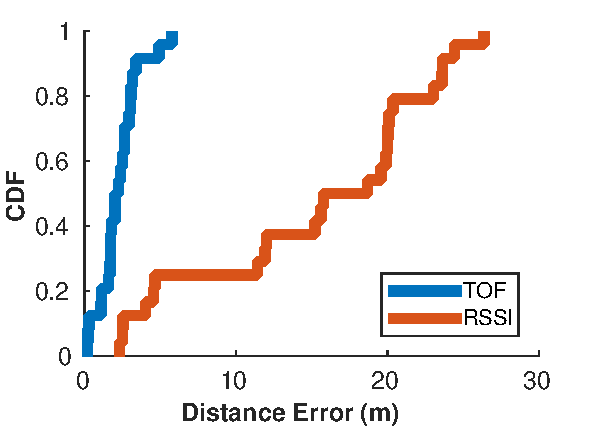
\includegraphics[width=.24\linewidth]{figures/PairwiseDistance.pdf}
} \hfill
\subfloat[]{
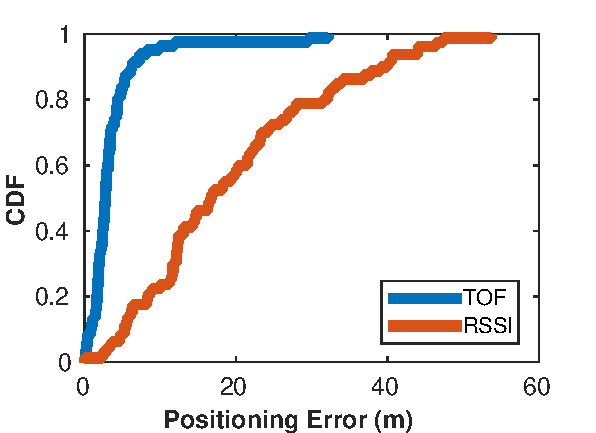
\includegraphics[width=.24\linewidth]{figures/PairwiseLocalization.pdf}
} \hfill
\subfloat[]{
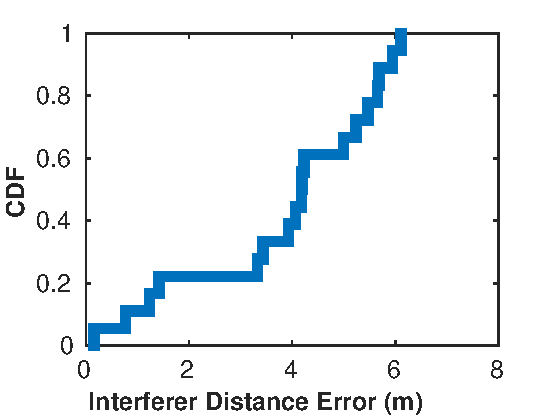
\includegraphics[width=.24\linewidth]{figures/InterfererDistance.pdf}
} \hfill
\subfloat[]{
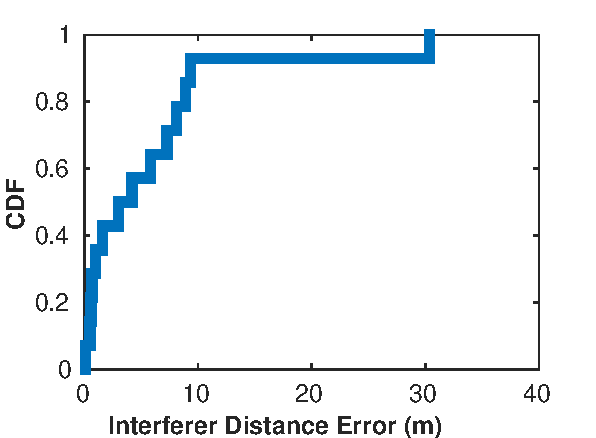
\includegraphics[width=.24\linewidth]{figures/InterfererLocalization.pdf}
}
\compactimg
\caption{Depicts localization error results. (a) shows the error in measuring the distance between two points between our system and the RSSI baseline, which corresponds to the localization error shown in (b). (c) shows the error of our system in locating distances to a receiving-limited client, corresponding with the localization error shown in (d).}
\label{fig:locres}
\end{figure*}


\subsection{Ranging and Localization} 
In this experiment, we evaluate the performance of our localization and ranging experiments. We conduct our experiments on both indoor and outdoor spaces in a large university campus. Our testbed considers  30 randomly chosen client locations with pairs of clients separated by distances of up to 40 meters in settings composed of walls, furniture and other obtrusions between the radios. The maximum signal range afforded by the RTL SDR is 40~m, owing to its hardware not being optimized for the 400 and 900 MHz ISM bands. We consider two types of clients: (1) Powered clients that have access to channel state-information; (2) Transmit-only clients that do not provide channel state information, to emulate interferers or unsophisticated battery-powered LP-WAN radios.  We compare our system with a baseline that uses RSSI-based fingerprinting~\cite{rssi}. Note that unlike the baseline, our system does not assume prior fingerprinting of the environment. 

\noindent\textbf{Locating Powered Devices}: We first measure the ranging error between pairs of clients that have access to channel-state information. Fig.~\ref{fig:locres}(a) depicts the CDF of the error in range between different pairs of devices whose distance is varied uniformly between 0-40 meters across randomly chosen locations in our indoor and outdoor testbeds. We observe a median ranging error of 2.21~m as against the RSSI baseline of 15.78~m. Fig.~\ref{fig:locres}(b) shows the CDF of the corresponding error in localization, recording a median error of 2.81~m as against the RSSI baseline of 16.81~m. We note that our approach achieves a superior accuracy in localization, despite the absence of prior fingerprinting of the environment, unlike the baseline. Further, while our maximum range with an RTL-SDR remains 40~m, owing to its general purpose design limited sensitivity to the 433~MHz/900MHz ISM bands, we believe our solutions error levels will remain consistent at full range with more sensitive RF front-ends optimized for these bands. 

\noindent\textbf{Locating Interfering or Battery-Powered Radios}: Next, we  evaluate localization performance of radios that do not provide us channel state information (CSI). We measure the time-difference of arrival between such radios and two powered clients in our testbed that provide channel state information from three vantage points. We then measure the error in distance corresponding to this time-difference in arrival. We repeat our experiments with the distance between the radio and our clients ranging from 0-40 meters across randomly chosen locations in our indoor and outdoor testbeds. Fig.~\ref{fig:locres}(c) depicts the CDF of this error  with a median of 4.19~m. Fig.~\ref{fig:locres}(d) shows the CDF of the corresponding error in localization, depicting a median error of 4.20~m. These results demonstrate that our approach can locate both interfering devices and transmit-only radios with an accuracy of a few meters, despite not having access to transmitted data or channel state information from such devices.   


\subsection{Link Performance at the Whitespaces}
While the above experiments were performed on the open ISM frequencies (the 433 MHz band and 902-928 MHz), our approach can benefit from the opening up of additional frequencies in the TV whitespaces. Fortunately, commercial LoRa radios are capable of operating on the 512-572 MHz whitespace frequency bands. \figref{freq-rssi} plots the RSSI gathered by transmissions from one LP-WAN radio to another at a distance of three meters in a sealed anechoic chamber (for regulatory reasons). We observe that LoRa radio experiences a gradual drop in performance in the whitespace band, as frequencies withdraw from the 433~MHz band. This is quite natural given that the radios are designed for the ISM bands, and no low-cost radio can be expected to perform optimally across a wide range of sub-GHz frequencies. However, this shows the promise of deploying large-scale LP-WAN testbeds using current LoRa technology in the whitespaces, particularly in dense low-range scenarios, such as apartment complexes, where spectrum shortages are commonplace.  

\begin{figure}
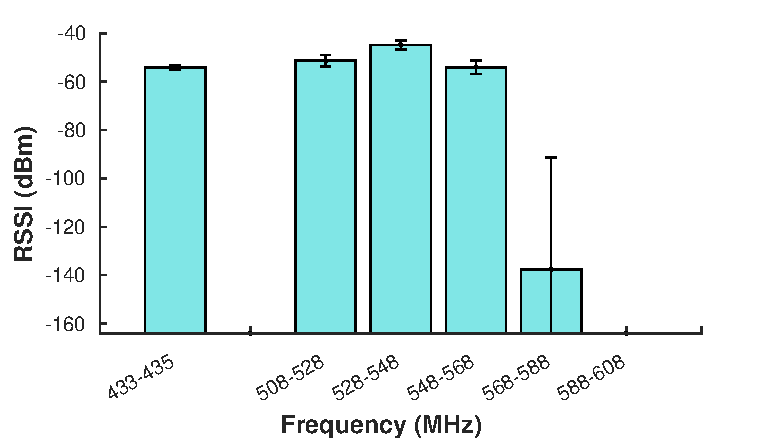
\includegraphics[height=4.5cm]{figures/Freq_vs_RSSI.pdf}
\caption{Depicts the RSSI and signal-to-interference plus noise ratio (SINR) for two LoRa devices 3~m apart across frequencies, including the unlicensed and TV whitespace bands. Demonstrates commercial LoRaWAN radios can receive and transmit on the TV whitespaces.}
\label{fig:freq-rssi}
\compactimg
\end{figure}

% \begin{figure}[!htb]
% \centering
% \includegraphics[width=0.4\textwidth]{figures/snr_vs_freq.jpg}
% \includegraphics[width=0.4\textwidth]{figures/rssi_vs_freq.jpg}
% \compactimg
% \caption{{Depicts the RSSI and signal-to-interference plus noise ratio (SINR) for two LoRa devices three meters apart across frequencies, including the unlicensed 433 MHz, 902-918 MHz and the 512-572 MHz TV whitespace band. Demonstrates commercial LoRaWAN radios can receive and transmit on the TV whitespaces.   }}
% \label{fig:lorabug-power-trace}
% \compactimg
% \end{figure}


\subsection{Campus-wide deployment}

\begin{figure}[!hbt]
\centering
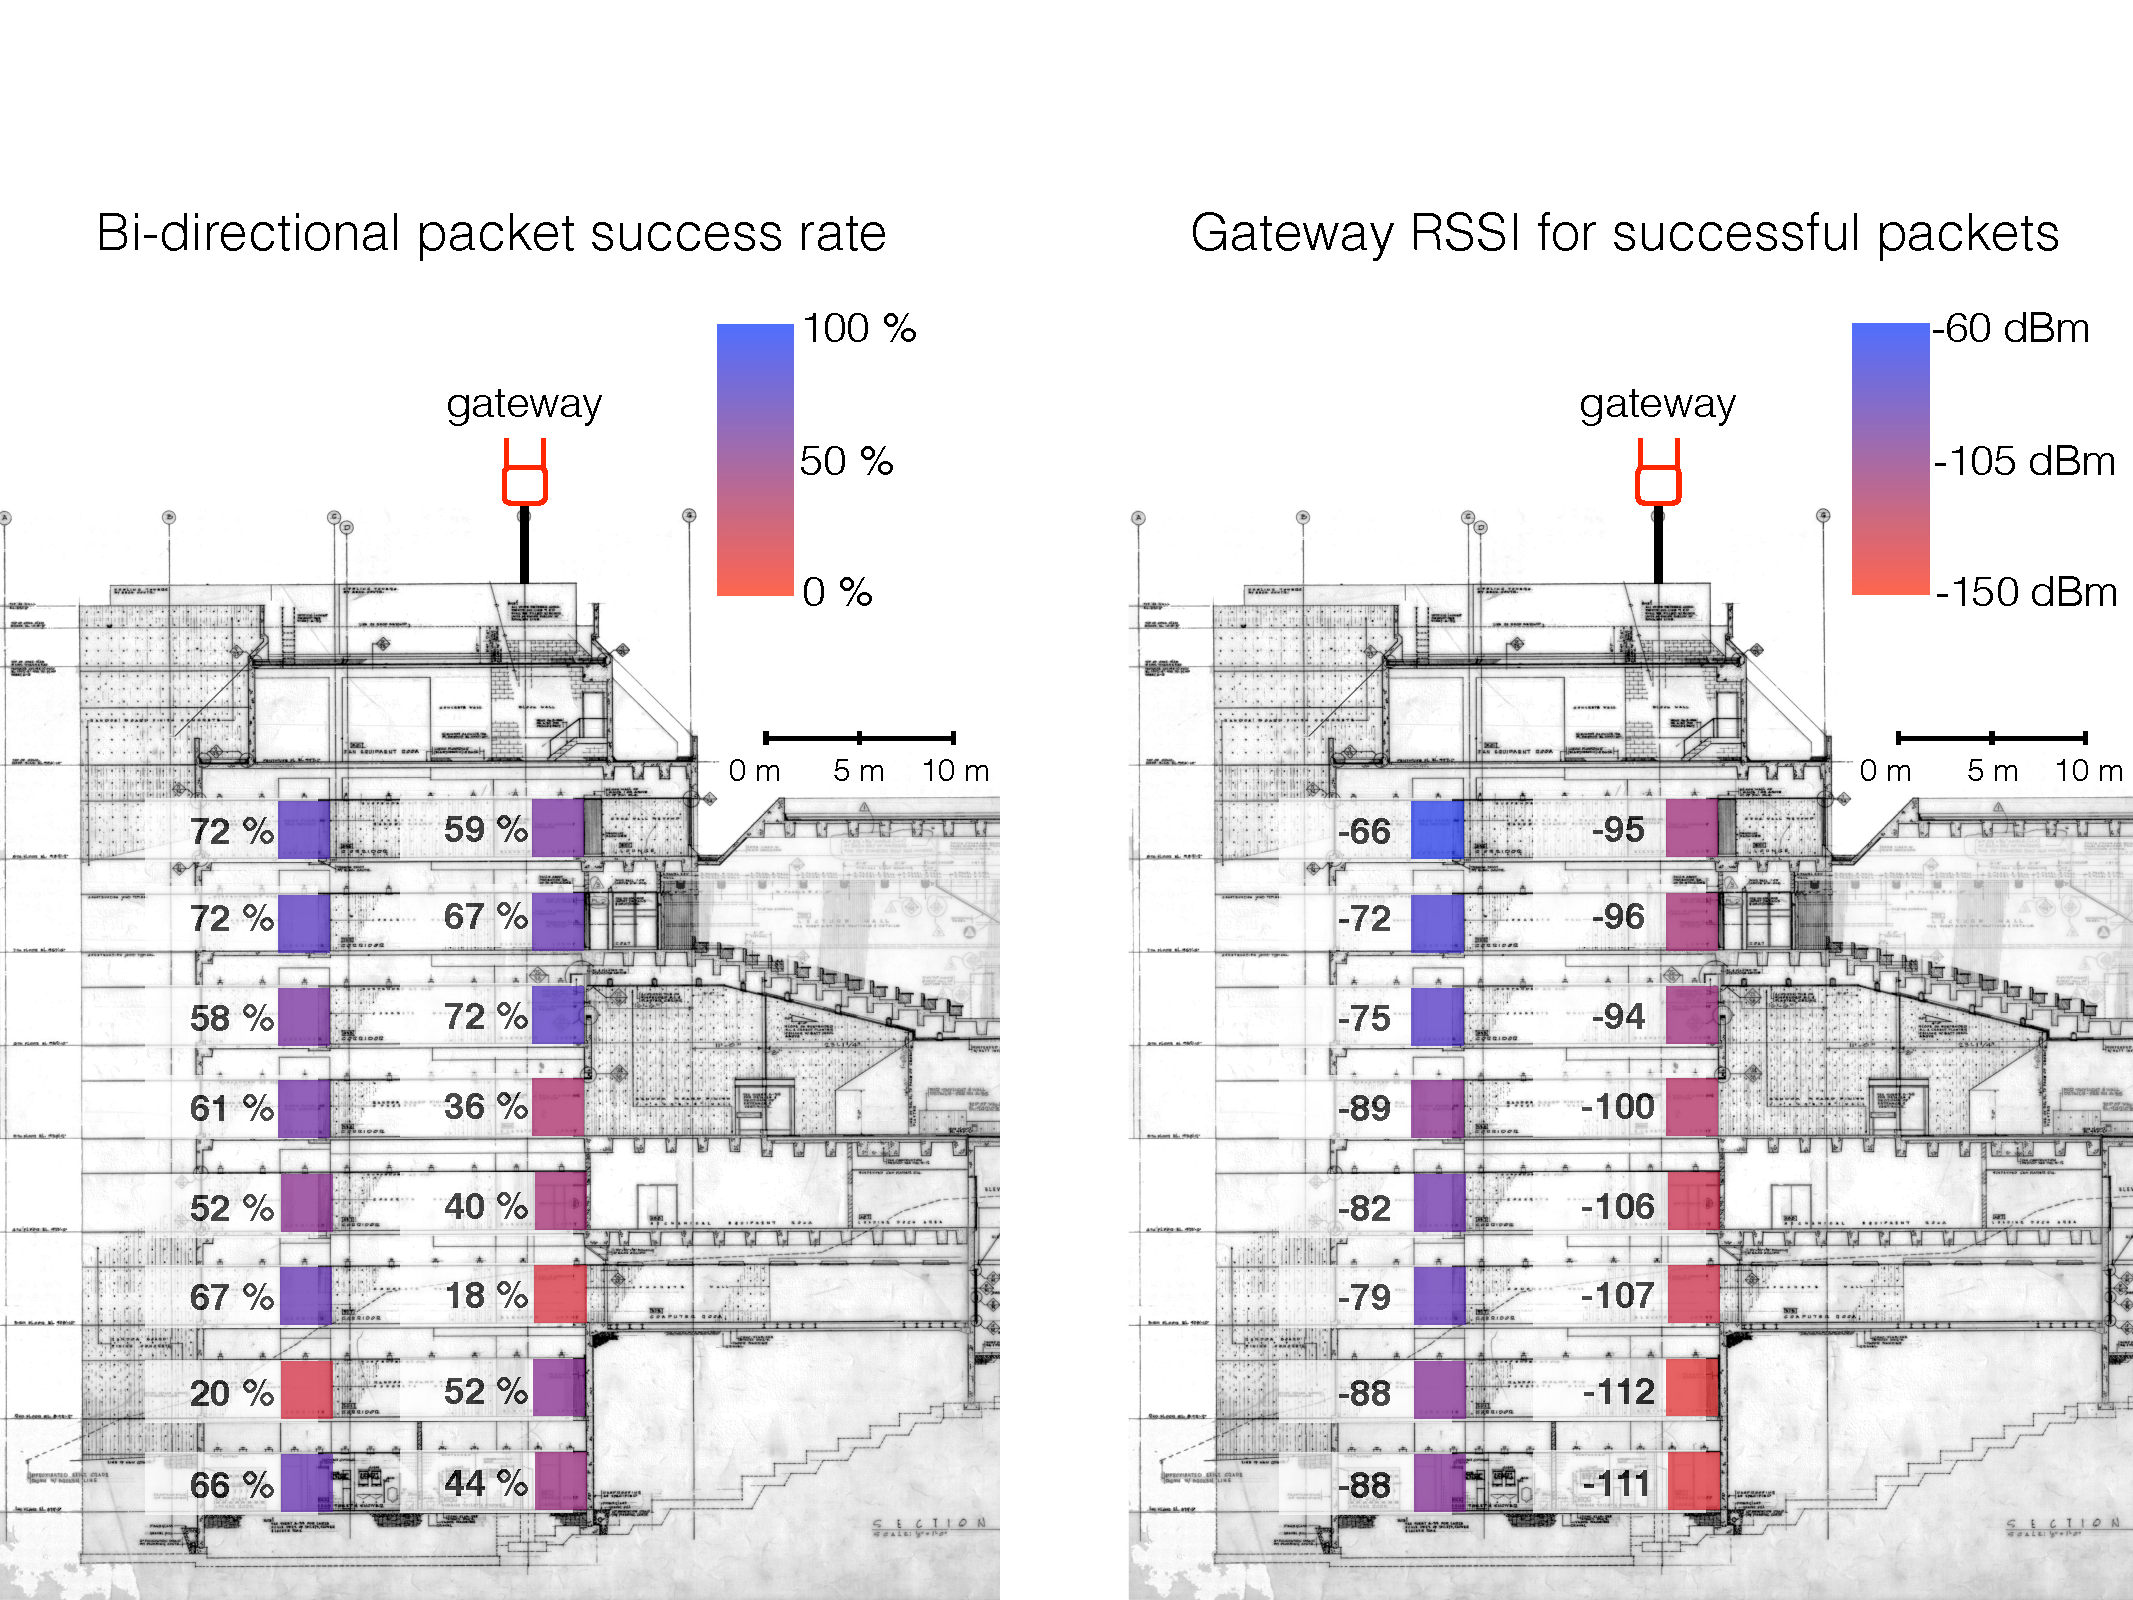
\includegraphics[width=\columnwidth]{figures/penetration_test_wean_cropped}
\compactimg
\caption{RF signal penetration experiments performed in a large poured-concrete building on campus. (left) shows the success rate for bi-directional packet exchange between end-node and gateway and (right) shows the RSSI at the gateway for successful transfers.}
\label{fig:penetration}
\compactimg
\end{figure}

% The remainder of this section describes the hardware and software components of our pilot network.

% \subsection{Server Back-end}

% The OpenChirp architecture shown in \figref{openchirp-arch} is a classical three-tiered design with sensor end-points at the bottom, followed by a gateway layer, and a server back-end that support applications at the top. All system configurations are carried out using a REST interface while devices that require more direct access to data like gateways or  processing agents communicate using a Publish-Subscribe layer.

% \noindent {\bf LoRaWAN Server:} The  LoRaWAN server is responsible for processing, decrypting and managing low-level LoRa communications. We extended the open-source LoRa server project~\cite{loraserver} that provides the underpinnings for MAC decisions like selection of the best downlink gateway, data rates and power levels for messages. The server exposes an MQTT-based Publish-Subscribe interface for both data and control messages making it easy to develop add-on modules. Most notably, we added support for our gateways hardware, our specific adaptive data rate algorithms and our global network management scheme.  

% \noindent {\bf Application Programming Interface (API):} External devices communicate with the OpenChirp network through two interfaces: (1) HTTP REST and (2) Publish-Subscribe (Pub-Sub). Client websites, mobile applications, management tools, etc. interface through an HTTP REST interface. The REST interface provides easy management of devices and their properties (location, metadata, functionality etc) as well as access to device time-series data. HTTP operations are managed by a server implemented in \textit{node}. Separating the OpenChirp API from the internal implementation of various services helps us create a modular architecture that also allows us to experiment with various components of the infrastructure.  

% \noindent {\bf Data Serialization:} A node can transfer limited data (tens of bytes per packet) over a LoRa connection due to a combination of communication restrictions and energy constraints. Data serialization gives us a flexible format to transfer various data types inside a single message structure. There are two observations with serialization: (1) the size for preregistered serialized messages is much smaller than if the same data were to be sent over raw key-value pairs and (2) existing serialization tools allow for faster processing and also enable static checking on serialized data. For the  serialization service, OpenChirp uses a simplified version of Google's Protocol Buffer~\cite{protobuff-google}, which can efficiently represent datatypes. When a new node is registered on the network, its serialization format is registered with the service. The service can then encode and decode data exchanged with the node.

% \noindent {\bf Timeseries and Meta-Data Storage:} A common application of IoT is identifying and acting on trends in the environment which requires data history. OpenChirp thus provides a time-series database (using \textit{InfluxDB}) that stores all data to and from end-devices. Applications and services can thus access historical data on-demand for a given time-interval in an efficient manner. This is accessible through our common REST API.  Some end-node and gateway properties like location, device type, capabilities, sensor sampling rates, closest gateway, etc. provide meaning and context to their data. These properties are stored as device metadata in an independent NoSQL (\textit{MongoDB}) database which also maintains access-control lists to regulate access to/modification of device data and meta-data. An LDAP authentication server is used to authenticate users that use the OpenChirp network. In our current deployment, students on campus can register and deploy their own devices with access control. If desired, they can share access with other account holders.


\begin{figure*}[!bt]
\centering
\subfloat{
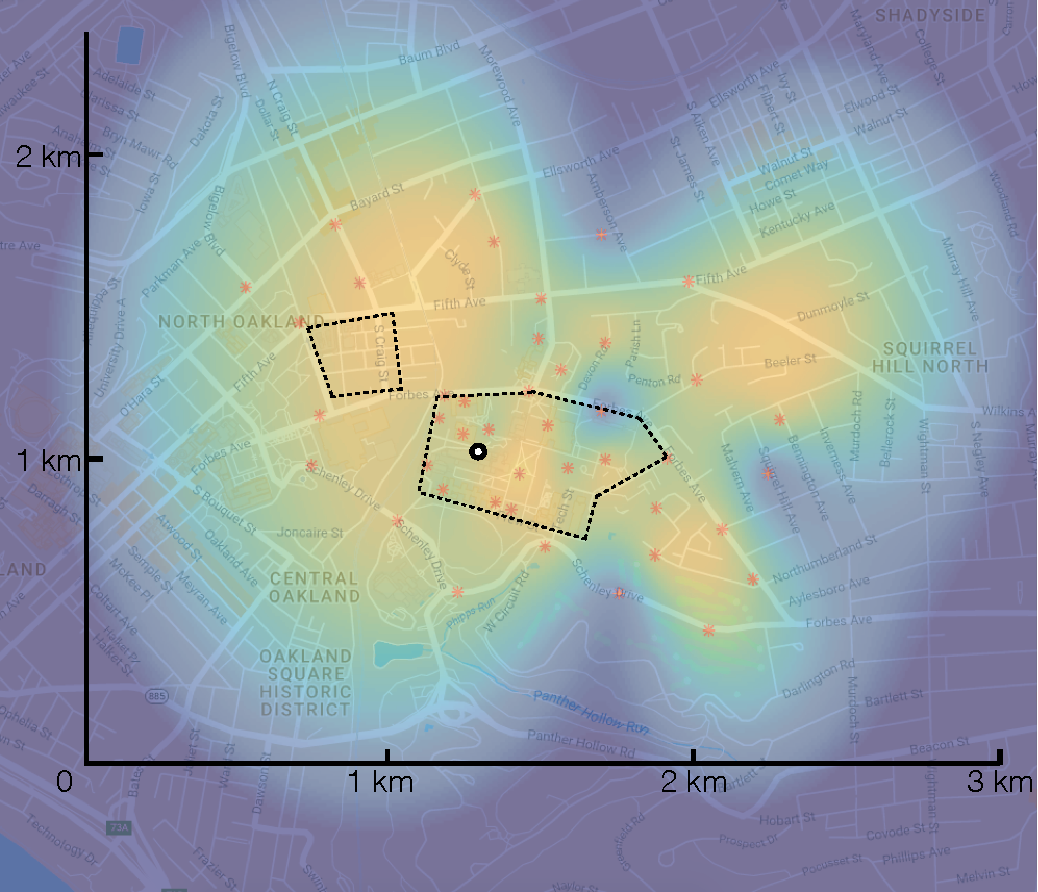
\includegraphics[height=4cm]{figures/cmu_heatmap_wean.pdf}
} \hfill
\subfloat{
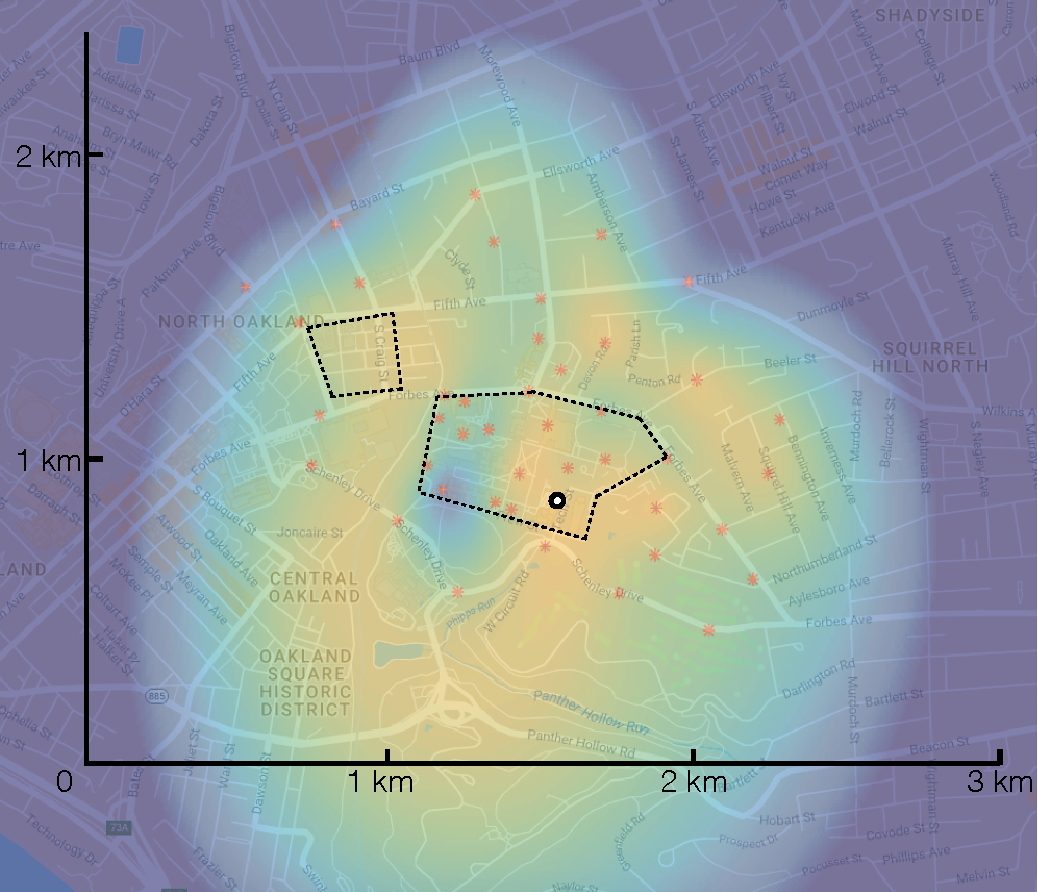
\includegraphics[height=4cm]{figures/cmu_heatmap_gsia.pdf}
} \hfill
\subfloat{
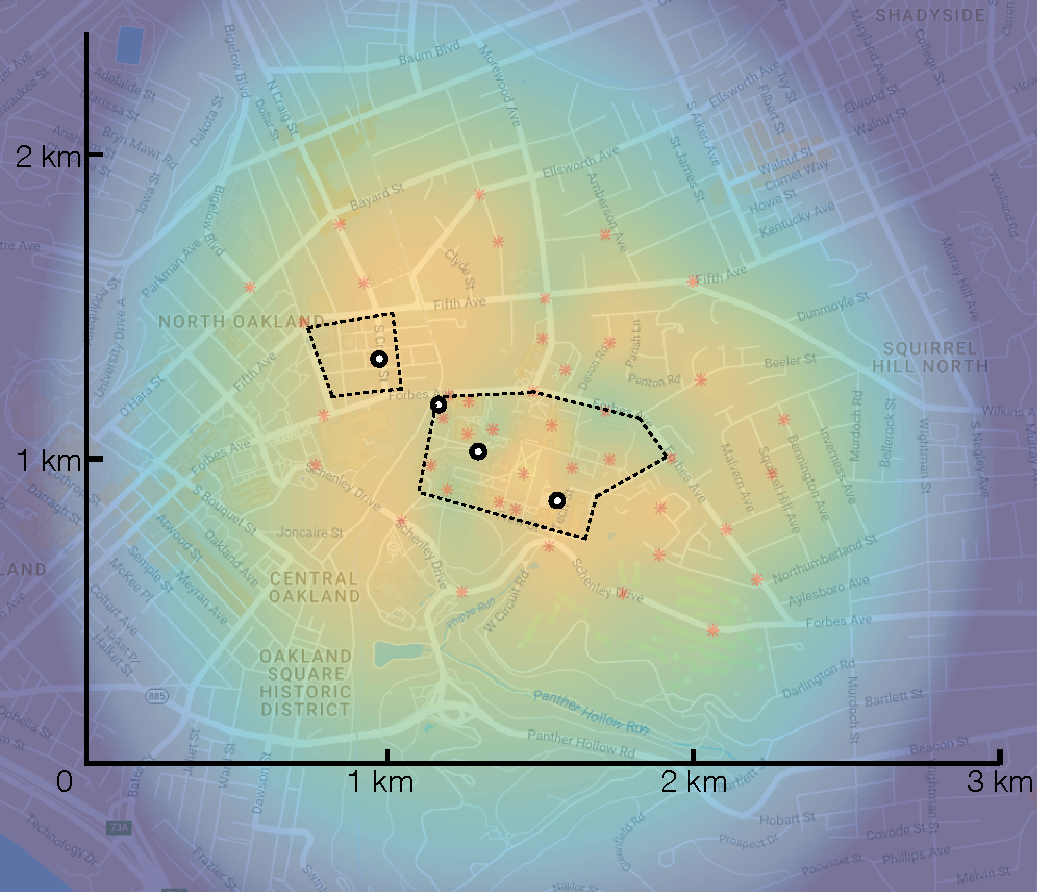
\includegraphics[height=4cm]{figures/cmu_heatmap_all_gw.pdf}
} \hfill
\subfloat{
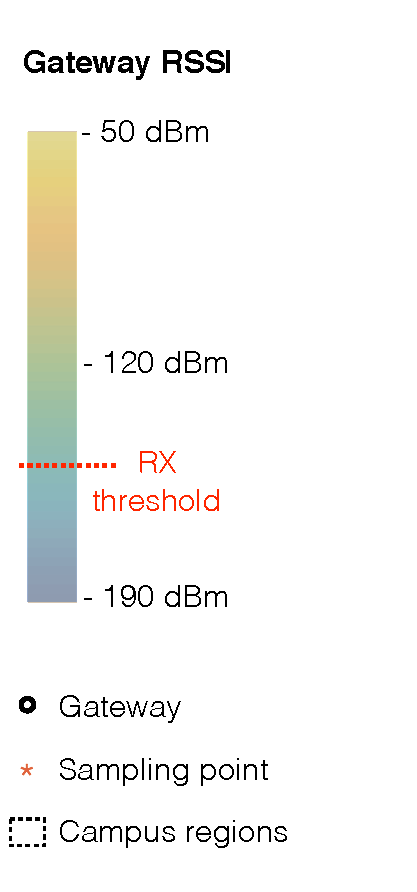
\includegraphics[height=4cm]{figures/heatmap_scale.pdf}
}
\compactimg
\caption{Network coverage in and around a large university campus campus with rooftop base stations.  (left) and (middle) show coverage areas of two candidate gateways and (right) depicts that of the combination of all gateways.}
\label{fig:wardrive}
\compactimg
\end{figure*}


We currently have a campus-wide LoRaWAN system available to the student body deployed at a large university campus.  The system consists of four rooftop gateways that support a variety of custom and commercially available sensing devices.  Our base stations were deployed to support coverage of the complete geographical area as well as signal penetration inside buildings. After installing our four gateways, we perform a set of coverage tests. The tests are performed with a LoRa end-node configured for uplink communications with 125 kHz channel bandwidth, data rate of 980 bits/s, spreading factor of 10 and coding rate of $4/5$. Downlink communications from the gateway used 500 kHz channels at 3900 bits/s. \figref{wardrive} shows the coverage heatmap based on the average received signal strength indicator (RSSI) of $\sim 12$ messages sent from each location. Though some regions may not be covered using one gateway (due to shadowing, attenuation, etc.), a combination of four gateways can successfully cover all major campus regions (>6 square km). We also explored the penetration inside of buildings. \figref{penetration} shows the signal penetration across multiple floors of a large 250,000 sq.ft. 9-story poured concrete building with a single gateway located on the roof. The packet success rate on the left is computed based on the number of complete bi-directional transfers ($\sim 60$ points in each left corridor, $\sim 15$ points in each right corridor). The image on the right shows the gateway RSSI of successful transfers. The traces obtained from this testbed were used to drive the trace-driven simulations described below.

\begin{figure}[bth]
\centering
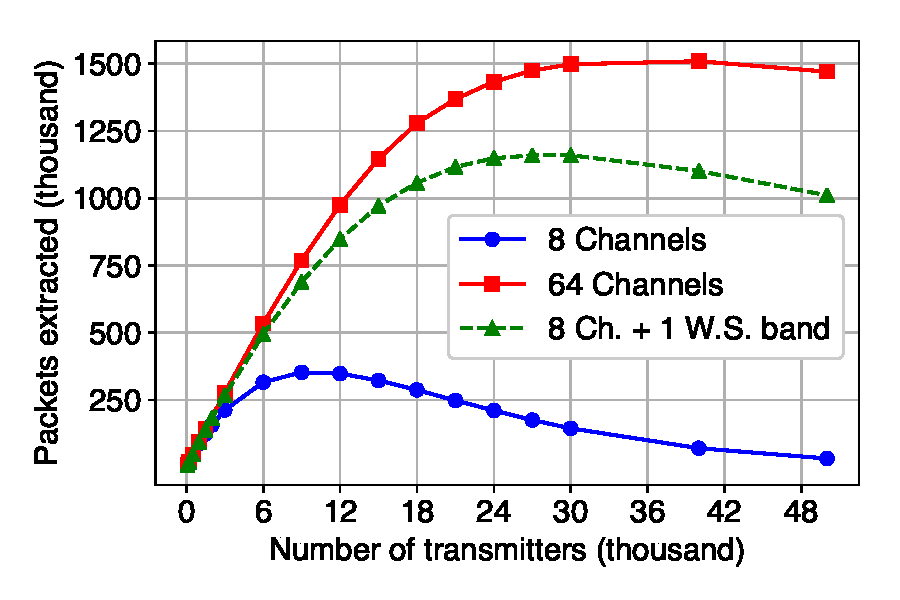
\includegraphics[width=0.8\columnwidth]{figures/8vs64channelvswhitespace}
\compactimg
\caption{Network throughput under increasing clients transmitting 20 byte packets every 15 minutes.  We see typical Aloha performance with a significant boost in capacity from a single White Space channel nearly matching the capacity of full 64-channel LoRaWAN gateway.}
\label{fig:ws-scaling}
\end{figure}

\section{Trace-Driven Simulations at Scale}
\label{sec:simulations}

Based on our micro-benchmarking experiments, we perform a set of trace-driven simulations to demonstrate the trends of our various approaches as the system scales.  \figref{ws-scaling} shows a baseline experiment simulating a week of time for a single base station in the middle of a 10$km$ by 10$km$ area with uniformly distributed nodes. The plot shows the effective throughput of the network as the number of clients increases using our additive interference model (spreading factor aware) as well as our more realistic capture effect model.  The 8-channel base-station represents the standard capacity of most current LoRa gateways.  The 64-channel base-station represents the capacity of our custom hardware which as one would expect servers approximately 8x more devices.  The 8-channel with a single white space band shows the potential of taking a normal gateway and equipping it with a white space radio system.  We see that each white space band provides about 80\% of the capacity of a 64-channel base station.  It is common for cities to have 1-3 of these bands free at any given time. 
 
\subsection{Base-Station Management}
\label{sec:bs-management}
As the number of base-stations increase, the network must manage them so as to minimize interference due to uncoordinated devices. \figref{coloring} shows a simulated deployment with 50 base-stations and varying number of uniformly distributed devices. The devices transmit on a single frequency in any of the 8 available frequency sets, without frequency hopping and are set at a spreading factor of 10. Frequency set allocations used by base-stations for uplink are generated using a BFS graph coloring strategy. Two base-stations are considered neighbors in a graph if a transmission from any device can be received by both of them. If the number of colors in the colored graph exceeds 8 (the number of frequency sets), we break links corresponding to the longest distances until the graph is 8-colorable. This approach provides a 5\% improvement to data extraction rate over a random frequency assignment approach.

\begin{figure}[bht]
\centering
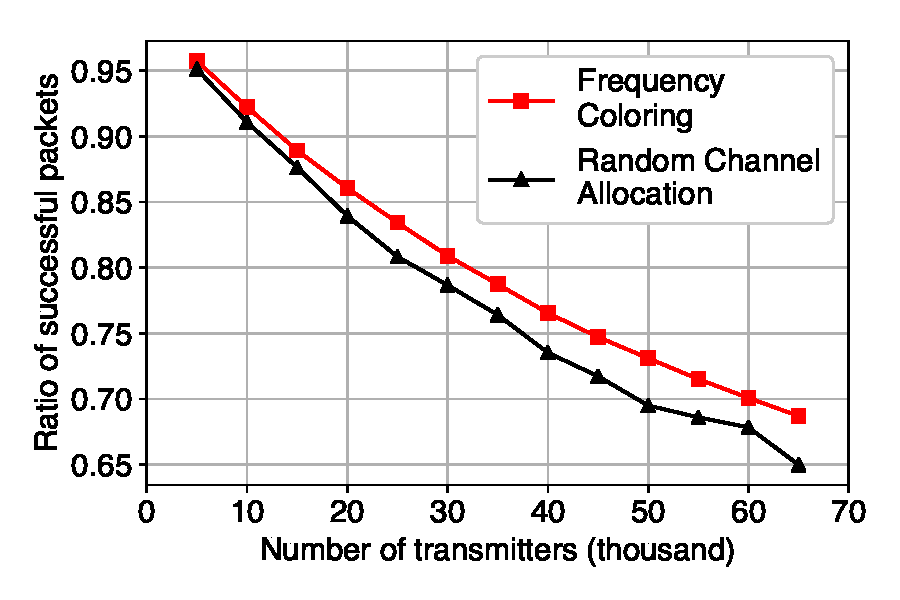
\includegraphics[width=0.8\columnwidth]{figures/RandomVsColoring}
\compactimg
\caption{Performance of scheduled gateway frequencies as compared to a greedy-allocation. As load increases we see up to a 5\% improvement in overall capacity.}
\label{fig:coloring}
\compactimg
\end{figure}


\begin{figure}
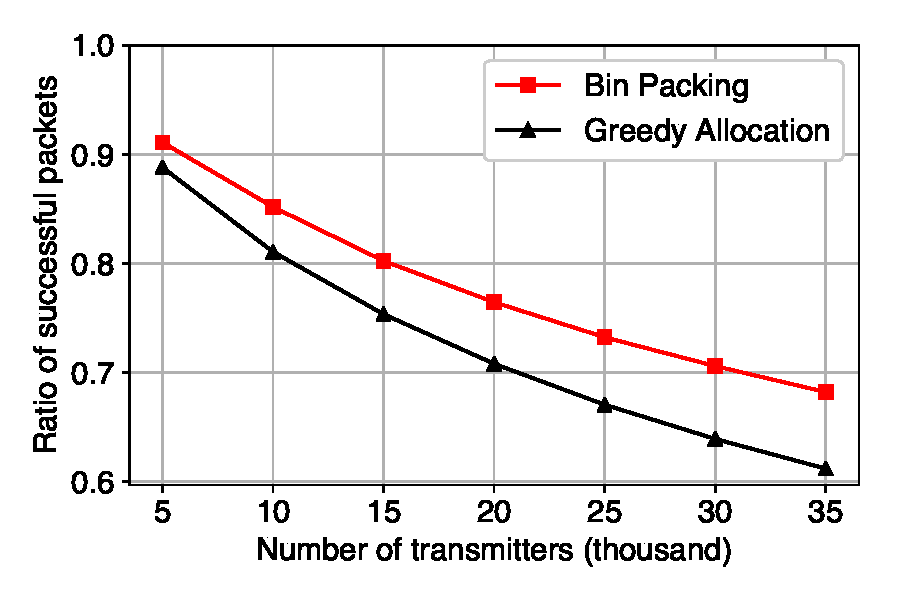
\includegraphics[width=0.8\columnwidth]{figures/binpacking}
\caption{Performance of our load balancing approach using joint channel and spread-factor load balancing vs the currently adopted Greedy allocation. With uniformly distributed nodes, we see a 7\% improvement in capacity. }
\label{fig:binpacking}
\compactimg
\end{figure}

\subsection{Client to Base-Station Association}
\figref{binpacking} shows the performance of our First-Fit bin packing heuristic, described in \secref{bs-assoc}, as compared with the commonly used greedy allocation scheme, that chooses to associate with the closest base-station. We simulate a dense deployment with 10 base-station (managed through coloring) in a small dense 1 $km^2$ area with other parameters identical to the previous section. As the density of nodes increases, the bin-packing scheme is better able to distribute the load between base-stations, reducing the number of collisions. The fact that we can utilize spreading factors to offload clients under heavy load is an interesting new technique for LP-WAN.

\begin{figure}
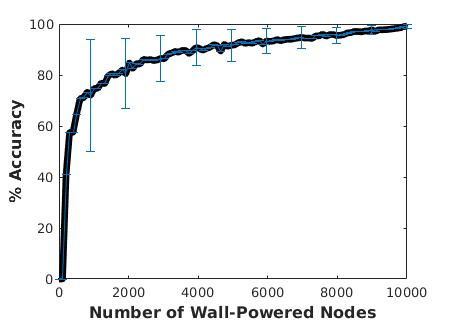
\includegraphics[height=4.5cm]{figures/InterferenceEstimation.jpg}
\caption{Shows the increasing accuracy in detecting the number of clients impacted by interference, using measurements from an increasing number of wall-powered nodes.}
\label{fig:intermit}
\end{figure}

\subsection{Interference Mitigation}\label{sec:resint}
This section demonstrates our system's ability to crowd-source interference detection using a large number of wall powered nodes in the network. We simulate a wide-area deployment of 10,000 clients a subset of them, chosen uniformly at random, being powered-nodes. We then place an interferer at a randomly chosen location and estimate the number of nodes impacted by this interferer, using the bounds of the powered nodes as described in Sec.~\ref{sec:interferemit}.

Fig.~\ref{fig:intermit} depicts the accuracy in the detection of impacted interferers as a function of the number of powered nodes. We observe that we can predict the impact of interference with $80\%$ accuracy with as few as $13\%$ of the clients in the network being wall-powered. 

\begin{figure}
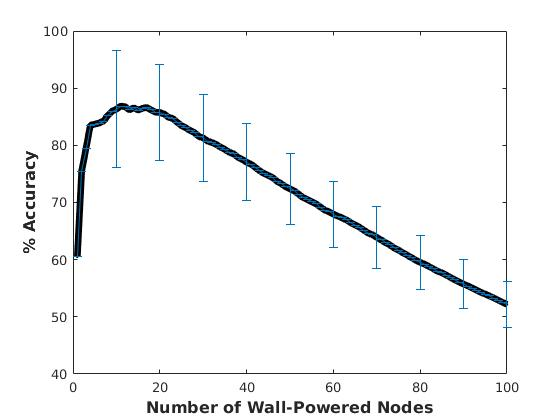
\includegraphics[height=4.5cm]{figures/BaseStationCounter.jpg}
\caption{Depicts the accuracy in detecting the number of clients a base station planned for a given location would serve, using measurements from an increasing number of wall-powered nodes in its vicinity. Using too many or too few nodes impacts accuracy. }
\label{fig:netplan}
\end{figure}

\subsection{Network Planning}
In this section, we evaluate the performance of the system in aiding base station deployment. We aim to calculate the number of nodes in range of a base station at a given location, prior to its deployment by using team of wall-powered clients to a emulate base station. We simulate a network of 10,000 nodes as before, with a 1\% of these nodes being powered. We assume the receive gain of powered nodes is $10\times$ weaker than that of the base station. We then calculate the accuracy of these nodes in tuning to the uplink and collectively measuring the number of clients in range of the base station.

Fig.~\ref{fig:netplan} shows the percentage accuracy of this quantity against the number of wall-powered nodes employed to emulate the base station. We note that while using too few powered nodes is inaccurate, using too many causes estimates from nodes that are well beyond the range of the planned base station to be employed in is range estimate. The results reveal that the Goldilocks zone is about 10\% of all powered nodes, among those closest to the base station, which ensured an accuracy of 80\% in our estimate. 

\section{Conclusion and Future Work}
\label{sec:conclusion-future-work}

{\color{red} Need new conclusions....}

% This paper presents a novel location-aware network management system for LoRa-class LP-WANs operating in unlicensed and whitespace frequencies. It presents an RF-based localization system that 
% stitches together information across frequencies to improve positioning accuracy of LoRa clients, even without access to their channel state information. We build on the localization framework to build a resource allocation system for LP-WAN that efficiently allocates wireless resources subject to FCC's regulatory constraints.  Our network-management system  is designed to be location-aware, exploiting live measurements to identify and respond to interference and help network managers plan changes to deployment. Our system was implemented and deployed in a large university campus and results from proof-of-concept experiments and large-scale trace-driven simulations are presented. In the future, we aim to expand our deployment to incorporate transmissions on the white spaces and are currently engaged in efforts to procure the relevant licenses. We also intend to integrate smart sensor devices currently deployed on-campus with LoRaWAN radios to evaluate our network management platform live and at-scale. 

\bibliographystyle{ACM-Reference-Format}
\bibliography{references} 

\end{document}
